\documentclass[a5paper, oneside,10pt]{article}

\usepackage[utf8]{inputenc}
\usepackage{amsmath}
\usepackage{caption}
\usepackage[spanish]{babel}
\usepackage{fontenc}
\usepackage{graphicx}
\graphicspath{{figures/}}
\usepackage{verbatim}
\usepackage{listings}
\usepackage[dvips]{hyperref}
\usepackage{fancyvrb,newverbs}
\usepackage{xcolor}
\usepackage{float}

\definecolor{bg}{gray}{0.93}
\definecolor{diffstart}{rgb}{0.1, 0.1, 0.5}
\definecolor{diffincl}{rgb}{0.1, 0.5, 0.1}
\definecolor{diffrem}{rgb}{1, 0, 0}

\lstdefinelanguage{diff}{
    frame=single,
    breaklines=true,
    basicstyle=\ttfamily\scriptsize,
    morecomment=[f][\color{diffstart}]{@@},
    morecomment=[f][\color{diffincl}]{+ },
    morecomment=[f][\color{diffrem}]{- },
    morecomment=[f][\color{diffstart}]{@@},
    morecomment=[f]{+++ },
    morecomment=[f]{--- },
  }
  
\lstdefinestyle{custom}{
  breaklines=true,
  frame=single,
  xleftmargin=\parindent,
  language=bash,
  showstringspaces=false,
  basicstyle=\ttfamily\scriptsize,
}

\newenvironment{cverbatim}
 {\SaveVerbatim{cverb}}
 {\endSaveVerbatim
  \flushleft\fboxrule=0pt\fboxsep=.5em
  \colorbox{bg}{\BUseVerbatim{cverb}}%
  \endflushleft
}

\newverbcommand{\cverb}
  {\setbox\verbbox\hbox\bgroup}
  {\egroup\colorbox{bg}{\box\verbbox}}

  
% Title Page
\title{Tutorial Git}
\author{Héctor Nieto Solana}

\begin{document}
 \maketitle
 \tableofcontents

 \clearpage
 
 \section*{Introducción}\addcontentsline{toc}{section}{Introducción}
 
  Este tutorial tiene como objetivo la familiarización con el entorno \verb+Git+ y la plataforma \verb+GitHub+. Está diseñado para seguir paso a paso, para su aprovechamiento óptimo a continuación se detalla la guía de estilos.
 
  Las explicaciones y desarrollo del tutorial se muestran en texto normal como éste.
 
  \begin{cverbatim}
Texto con este formato corresponde a los comandos a escribir
literalmente en el terminal de tu sistema operativo. 
  \end{cverbatim}

  Cuando el texto aparezca rodeado por unos corchetes \cverb+<texto_libre>+ indica que el texto a introducir es libre a discrección del alumno.
  
  \begin{lstlisting}[style=custom, caption=Ejemplo de salida retornada por un comando]
El texto dentro de un recuadro como este indica la salida retornada tras ejecutar un comando
  \end{lstlisting} 

 \clearpage

 \section{Primeros pasos}

  \subsection{Creación de una cuenta de GitHub}\label{sec:github_login}
    GitHub es una plataforma online de repositorios \verb+Git+ que actualmente forma parte de la matriz de Microsoft. Para bien o para mal\footnote{Bill Gates se está metiendo dentro de tí no sólo a través de las vacunas}, GitHub es probablemente la plataforma más utilizada para compartir y trabajar online con código abierto, por lo que en este curso nos centraremos en esta plataforma. No obstante, hay otras plataformas alternativas para almacenar tus códigos en la nube como pueden ser \href{https://about.gitlab.com}{GitLab}, \href{https://bitbucket.org}{BitBucket}, e incluso tú o tu compañia/departamento puede tener tu propia plataforma \verb+Git+ para la gestión de software y código. Un último comentario antes de ponernos en faena es que para trabajar con \verb+Git+ no es necesario utilizar GitHub, sin embargo para trabajar con GitHub sí necesitas usar \verb+Git+. 
    
    En tu explorador web favorito teclea \url{github.com}´y regístrate introduciendo tus datos. GitHub ofrece cuentas gratuitas con un número limitado de respositorios públicos y/o privados por lo que en princpio es más que suficiente para las tareas diarias que necesitarás para este tutorial y también para el futuro. Es importante que elijas un nombre de usuario fácil de memorizar y de identificar por otros, ya que tu espacio GitHub será \verb+https://github.com/<nombre_de_usuario>+\footnote{Gonzalo, a no ser que busques trabajar para Cerezo mejor evita la tentación d ponerte como usuario oleoleolecholosimeone}
    
  \subsection{Instalación de Git}
    En casi todo este curso vamos a trabajar mediante líneas de comandos de \verb+Git+. En primer lugar tendremos que instalar \verb+Git+ en caso de que no esté aún instalado en tu equipo. Sigue las instrucciones adecuadas según el sistema operativo que tengas: 
    
    \begin{itemize}
      \item MacOs: Teclea en un terminal
        \cverb|brew install git|

      \item Windows: Pincha en el siguiente enlace. 
      
      \url{https://git-scm.com/download/win}
      
      La descarga e instalación debería ser automática
        
      \item Linux Debian. Teclea en un terminal
        \cverb|sudo apt install git-all|
    \end{itemize}
    Ahora sólo un par de pasos para la configuración básica de \verb+Git+ en tu PC. Con el fin de que todos los cambios y versiones que realices queden registrados a tu nombre teclea estos dos comandos:
    \begin{cverbatim}
git config --global user.name <nombre_de_usuario>
git config --global user.email <email>
    \end{cverbatim}
      
    Como tenemos una cuenta de GitHub lo mejor es usar el mismo nombre de usuario y el mail que has utilizado para registrarte. El \emph{keyword} \cverb+--global+ está especificando que la variable user.name y user.email son aplicables a todo el entorno git, es decir no hace falta que más adelante especifiques de nuevo un usuario y un correo electrónico cada vez que crees un repositorio en tu PC\footnote{Si no pones --global las configuraciones que hagas se aplican sólo al repositorio en el que te encuentres}.

  \section{Iniciación a Git}
    \subsection{Crea tu primer repositorio}
    \begin{enumerate}
      \item Abre un terminal y navega a la carpeta donde quieras crear el repositorio\footnote{usa cd para ir cambiando de carpetas}. Para este ejercicio recomiendo usar una carpeta vacía pero en el futuro puedes usar una carpeta donde tengas algún código ya existente. 
      
      \item Una vez estés en la carpeta de destino teclea
      
      \cverb+git init+
    
      Un mensaje similar a este aparece diciendo que has creado un nevo repositorio vacío.
      
      \begin{lstlisting}[style=custom, caption=Mensaje al inicializar git]
  Initialized empty Git repository in <carpeta_actual>
      \end{lstlisting}
      
      \item Si te fijas de nuevo en tu carpeta de trabajo, \verb+Git+ ha creado una subcarpeta llamada ``\verb+.git+'' con todos los archivos que requiere el sistema. Si no la ves no entres en pánico, por defecto esta carpeta está oculta\footnote{En Linux todos los archivos y carpetas que comienzan con un punto (``.'') son ocultos}
    
      \begin{lstlisting}[style=custom, caption=Archivos y subcarpetas por defecto del sistema .git]
  $ ls -lha
    total 40K
    drwxrwxr-x 7 hector hector 4,0K may  7 11:01 .
    drwxrwxr-x 3 hector hector 4,0K may  7 11:01 ..
    drwxrwxr-x 2 hector hector 4,0K may  7 11:01 branches
    -rw-rw-r-- 1 hector hector   92 may  7 11:01 config
    -rw-rw-r-- 1 hector hector   73 may  7 11:01 description
    -rw-rw-r-- 1 hector hector   23 may  7 11:01 HEAD
    drwxrwxr-x 2 hector hector 4,0K may  7 11:01 hooks
    drwxrwxr-x 2 hector hector 4,0K may  7 11:01 info
    drwxrwxr-x 4 hector hector 4,0K may  7 11:01 objects
    drwxrwxr-x 4 hector hector 4,0K may  7 11:01 refs
      \end{lstlisting}
    
      No vamos a entrar en detalle sobre la estructura y contenido de esta carpeta ya que es parte del sistema interno de \verb+Git+. Simplemente remarcar que todos los cambios y versiones que hagas en tu futuro código, quedarán registrado dentro de esta carpeta, por lo que nunca la borres. Por otro lado, si quieres borrar un proyecto de \verb+Git+, no tienes más que borrar esta subcarpeta.
    
    \item En la carpeta donde creaste el repositorio vacío crea o guarda un archivo de texto con este texto\footnote{He omitido los acentos a conciencia para evitar usar caracteres especiales}
    \begin{cverbatim}
mi primera linea de codigo
    \end{cverbatim}
    
    \item Teclea ahora \cverb+git status+ para ver el estado actual de tu repositorio. El sistema te retornaría un mensaje similar a este:
    
    \begin{lstlisting}[style=custom]
On branch master

No commits yet

Untracked files:
  (use "git add <file>..." to include in what will be  committed)
	archivo_1.txt

nothing added to commit but untracked files present (use "git add" to track)
    \end{lstlisting}
    En resumen \verb+Git+ te está diciendo que en la carpeta hay un arhivo nuevo (en el ejemplo llamado \verb+archivo_1.txt"+) que aún no está en seguimiento.

    \item Añade este archivo al sistema tecleando
    \begin{cverbatim}
git add <nombre_del_archivo>
    \end{cverbatim}
    y vueve a teclear \cverb+git status+, ahora aparecería un mensaje similar a este:
    
    \begin{lstlisting}[style=custom]
On branch master

No commits yet

Changes to be committed:
  (use "git rm --cached <file>..." to unstage)
	new file:   archivo_1.txt
    \end{lstlisting}

    \item Registra los cambios realizados como una nueva versión
    \begin{cverbatim}
git commit -m 'My first commit'
    \end{cverbatim}
    
    y de nuevo teclea \cverb+git status+. Ahora te dice que tu espacio de trabajo está limpio y no tienes ningún otro cambio por confirmar/descartar

    \begin{lstlisting}[style=custom]
On branch master
nothing to commit, working tree clean
    \end{lstlisting}
    
    \end{enumerate}
    
    \subsection{Crear repositorio en GitHub}
      Para esta parte es necesario que ya tengas un usuario registrado en GitHub, por lo que si  aún no lo has hecho sigue los pasos mostrados en la sección \ref{sec:github_login}.
      
      \begin{enumerate}
       \item Ve a tu espacio GitHub con tu navegador internet \url{https://github.com/<usuario>} e identifícate pinchando en \verb+Sign In+ en la esquina superior derecha con tu contraseña\footnote{Según la configuración de Cookies de tu navegador es posible que al entrar en tu espacio ya estés registrado/a}.
       \item Para crear un nuevo repositorio puedes pinchar bien en el icono \cverb!+! de la esquina superior derecha o pinchando en primer lugar la pestaña de \cverb+Repositories+ y luego el icono verde \cverb+New+. Un cuadro de diálogo como éste debería aparecer:
       
       \begin{figure}[H]\centering
        \hspace{-1cm}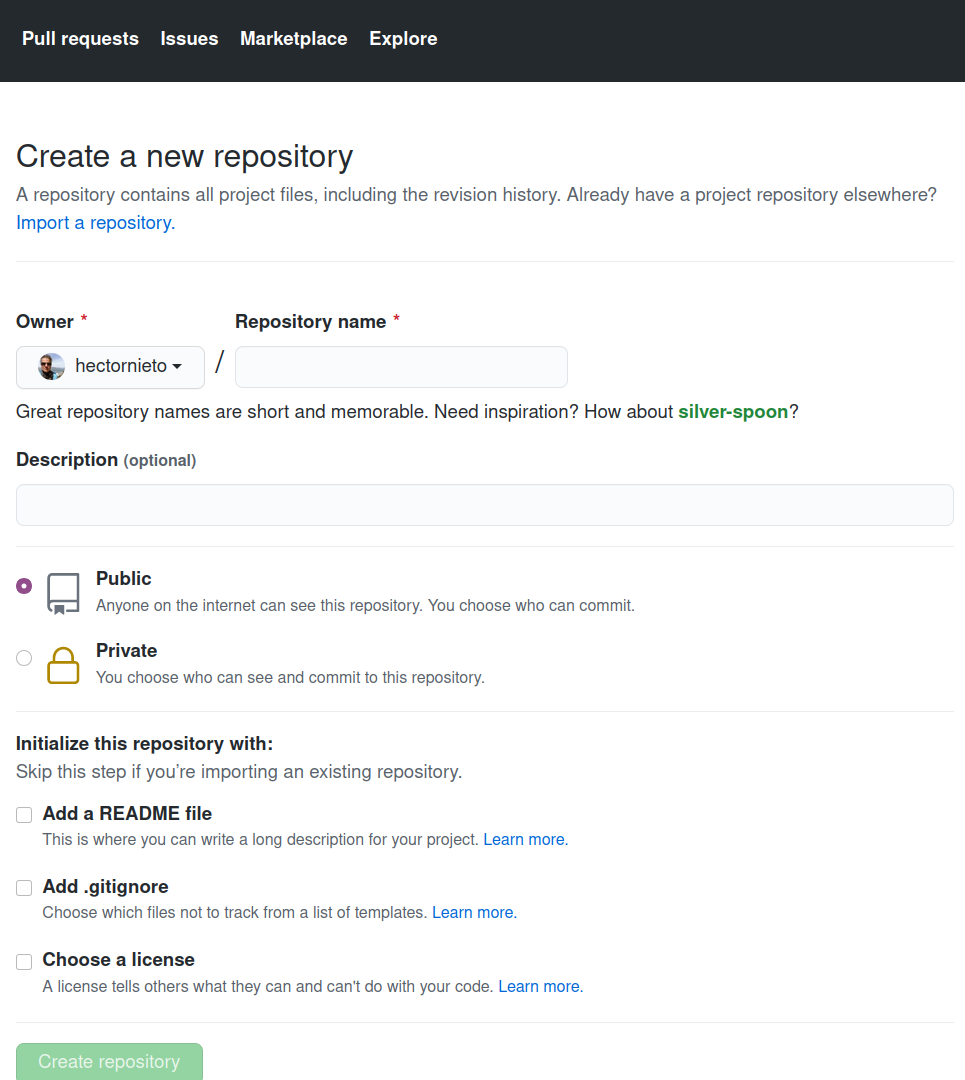
\includegraphics[width=1.2\columnwidth]{github_create_new_repo}
       \end{figure}
       
       \item Para este primer caso vamos a crear un repositorio donde vamos a subir nuestro ejercicio. Así que lo nombraremos como \cverb+primeros_pasos+.
       
       \item La descripción suele ser una línea o dos de texto libre que resuma tu repositorio/software. Algo así como ``Voy a disfrutar tanto de este curso que he decidido subirlo a GitHub'', o este otro ``La UAH necesita una prueba de que he realizado el curso satisfactoriamente por lo que colgaré mis tareas en GitHub esto como evidencia''
       
       \item Ahora, como no queréis que vuestros compañeros de curso se copien de tu ejercicio supremo, vamos a seleccionar que nuestro repositorio sea privado\footnote{Actualmente el plan gratuito de GitHub admite crear repositorios tanto públicos como privados ilimitados}. Esto implicará que nadie puede ver tu código a no ser que le des permiso expreso como colaborador (lo haremos más adelante).
       
       \item Deja sin marcar las opciones \cverb+Add a README file+, \cverb+Add gitignore+ y \cverb+Choose a license+, ya que en la siguiente tarea vamos a importar nuestro repositorio local ya existente.
       
       \item Finalmente pincha en el botón verde \cverb+Create repository+ en muy poco tiempo te aparecerá una ventana explicándote los siguientes pasos/opciones que puedes hacer para importar tu repositorio. En nuestro caso usaremos la segunda opción (pero más adelante)
       
       \item Antes de terminar con esta parte, una cosa importante de los repositorios privados es controlar quién puede acceder a ellos. Vais a añadirme como colaborador de este repositorio que acabáis de crear, para ello pinchad en \cverb+Settings+ y depués en la barra izquierda en la segunda opción \cverb+Manage Access+. Os aparecerá esta pantalla, tras lo cual pincháis en el botón verde de \cverb+Invite a collaborator+

       \begin{figure}[H]\centering
        \hspace{-1cm}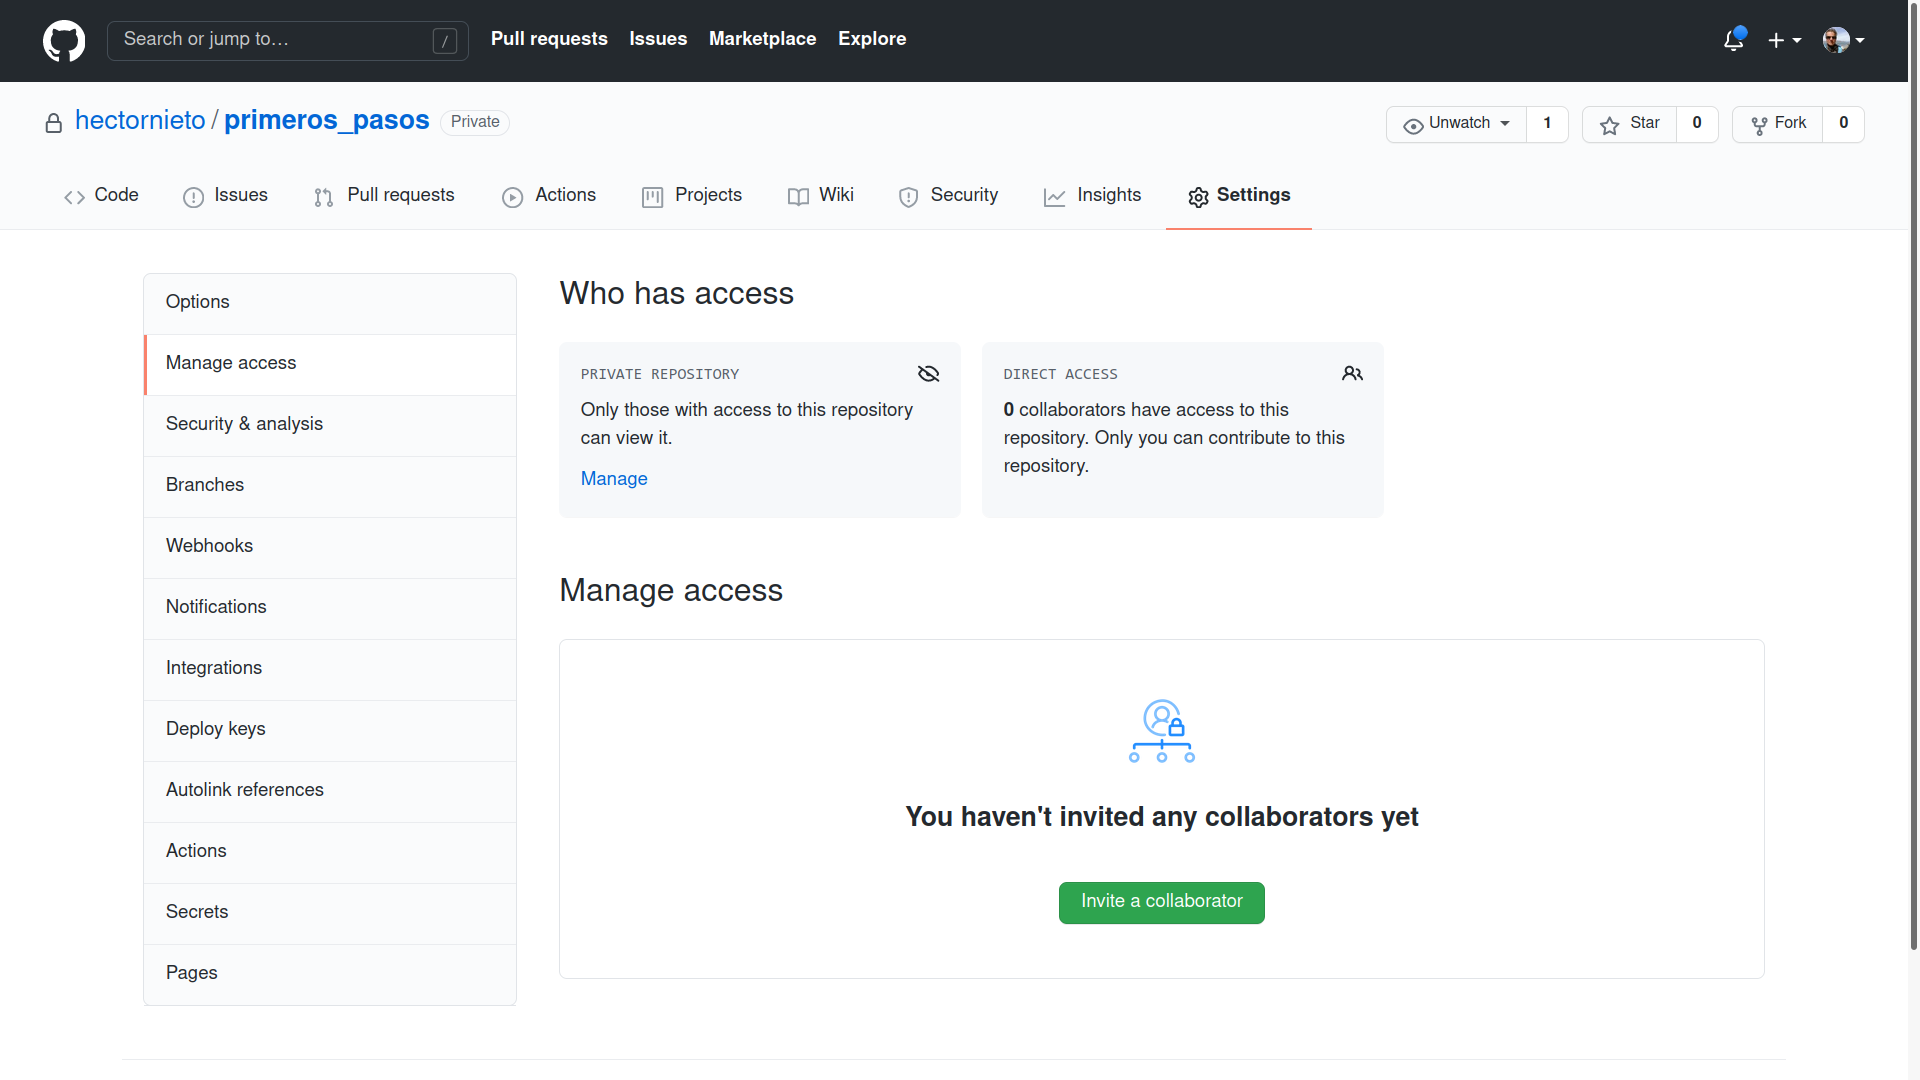
\includegraphics[width=1.2\columnwidth]{github_add_collaborator}
       \end{figure}
       
       En el recuadro tenéis que buscarme por usuario \cverb+hectornieto+, en caso de duda u os salgan otros usuarios similares, mi usuario tiene mi foto, o alguien parecido a mí con gafas de sol con el Golden Gate de fondo. De este modo sólo tu y yo podremos ver tu repositorio en GitHub, y podré ademas sugerirte cambios a través de un \cverb+Pull Request+.
      \end{enumerate}
       
       En cualquier caso, te recomiendo que generes otro repositorio desde GitHub y en este caso marques estas tres casillas para que experimentes lo que hace GitHub:
       
       \begin{itemize}
        \item Marcar la opción de \cverb+Add a README file+ creará en el la carpeta raíz del repositorio un archivo vacío README.md. Éste es un archivo ASCII de texto que GitHub lee y lo incorpora como descripción completa del repositorio. El archivo README.md (y por defecto la extensión \verb+md+ se basa en la edición en Markdown, una serie de etiquetas muy sencillas que permite darle formato al texto (secciones, hipervínculos, viñetas, ...). Para más información de por qué es útil el README.md y qué información incluir pincha \href{https://github.com/18F/open-source-guide/blob/18f-pages/pages/making-readmes-readable.md}{aquí}. Para saber más sobre escritura en Markdown ve a \url{https://www.markdownguide.org/getting-started/}. Si quieres ver un ejemplo de un README.md puedes ir a alguno de mis repositorios públicos, p.ej \url{https://github.com/hectornieto/pyTSEB/README.md}
       
        \item Marcar la opción de \cverb+Add gitignore+ te permite elegir una de las plantillas, que te aparecerá en el menú desplegable, según el lenguaje de programación habitual que utilices. \cverb+.gitignore+ es un archivo (oculto) que puede estar en la carpeta raíz de cada repositorio \verb+Git+ y que dice a \verb+Git+ qué archivos, dentro de las carpetas y subcarpetas del repositorio, va a ignorar a la hora de detectar los cambios. Este archivo es muy útil en la mayoría de los casos ya que la mayoría de los lenguajes de programación generan (bien al compilarse o a ejecutarse) un gran número de archivos (por ejemplo \verb+.pyc+ en Python o \verb+.o+ en C) que no son parte del código fuente y por lo tanto no merece la pena realizar un seguimiento sobre ellos.
       
        \item Para finalizar, \cverb+Choose a license+  añadirá   también automáticamente un arhivo con el texto de la licencia y un mensaje en la página principal destacando la licencia bajo la que está el repositorio. En el futuro para tus repositorios, sobre todo los públicos, es recomendable elegir cuidadosamente la licencia. En este caso este curso (todo el tutorial y los ejemplos) los he generado bajo la licencia \cverb+Creative Commons Zero+ por lo que tienes libertad total para usarlo y distribuirlo para lo que te plazca.
       
        \item Finalmente si pinchas ahora en el botón verde \cverb+Create repository+ en muy poco tiempo te aparecería la ventana un repositorio GitHub, pero ya con contenido y un primer commit, con los tres archivos mencionados anteriormente:
       
       \begin{figure}[H]¯
        \hspace{-1cm}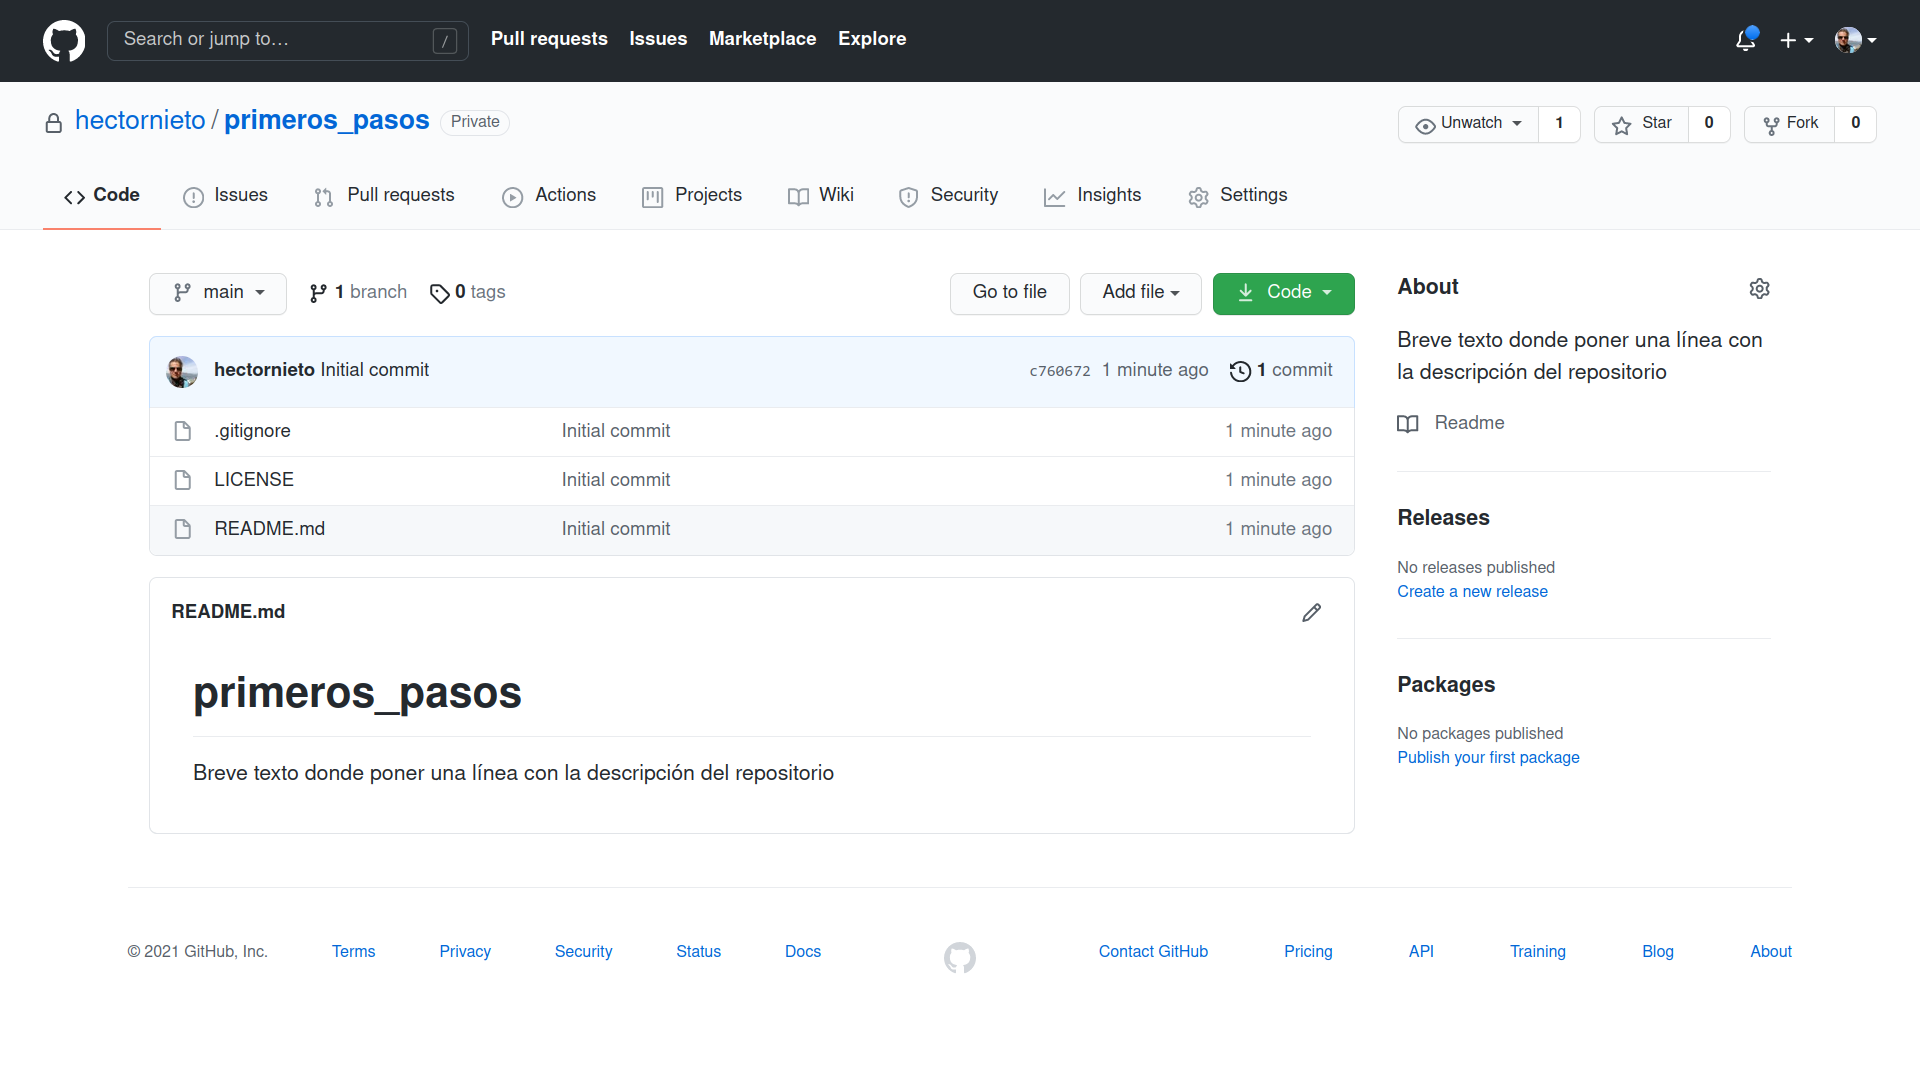
\includegraphics[width=1.2\columnwidth]{github_new_repo}
       \end{figure}
       
        \item Puedes navegar y visualizar ahora el contenido de los tres archivos y familiarizarte un poco con el entorno de trabajo de GitHub. En el que puedes incluso editar código y archivos, aunque siempre es recomendable trabajar en local, editando los arhivos en tu PC, para luego sincronizar el repositorio local con el remoto. 
        
        Hay un gran número de pestañas en cada repositorios, pero en realidad, tan sólo usarás el 99\% del tiempo la pestaña de \cverb+Code+, \cverb+Settings+ e \cverb+Insights+, en ese orden de importancia. Luego en menor medida, y lo veremos más adelante la pestaña de \cverb+Pull Requests+.
       \end{itemize}
       
    \subsection{Añadir y sincronizar repositorio remoto}\label{sec:sincronizar}
      Ahora que tenemos el repositorio remoto vamos a añadirlo a nuestro repositorio local y sincronizar el contenido de ambos, con el fin de tener en la nube lo que hemos hecho hasta ahora. 
      \begin{enumerate}
       \item Vuelve a la terminal y a la carpeta donde has estado trabajando con \verb+Git+ y teclea

        \hspace{-3cm}\cverb+git remote add <alias_del_remoto> https://github.com/<usuario>/<repositorio>+
       
       \cverb+<alias_del_remoto>+ puede ser cualquier nombre que le quieras dar, el nombre más típico que los usuarios dan es \cverb+origin+, como indicativo que la versión en la nube es el origen de todas, ya que es la única accesible a todos los usuarios o colaboradores, pero también se suele usar como nombre \cverb+remote+ o \cverb+upstream+. \cverb+<usuario>+ es tu usuario github y por último \cverb+<repositorio>+ es el nombre del repositorio que le dimos en GitHub (\cverb+primeros_pasos+)
       
       \item Finalmente vamos a subir todo lo que tenemos hasta ahora con el siguiente comando:
       
       \cverb+git push -u <alias_del_remoto> <branch>+
       
       donde \cverb+<alias_del_remoto>+ es el nombre que le dimos con el comando \cverb+git remote add+, y \cverb+<branch>+ es la rama que queremos subir (\cverb+master+ generalmente). La opción \cverb+-u+ es para que genere una nueva rama en el remoto y la asigne esa rama al seguimiento de la rama local actual, por lo que sólo es necesario incluir esta opción la primera vez que subamos una nueva rama al remoto. \verb+Git+ retorna un mensaje parecido a este si todo se ha subido adecuadamente:
       \begin{lstlisting}[style=custom]
Username for 'https://github.com': hectornieto
Password for 'https://hectornieto@github.com': 
Enumerating objects: 12, done.
Counting objects: 100% (12/12), done.
Delta compression using up to 4 threads
Compressing objects: 100% (6/6), done.
Writing objects: 100% (12/12), 1.03 KiB | 350.00 KiB/s, done.
Total 12 (delta 0), reused 0 (delta 0)
To https://github.com/hectornieto/primeros_pasos
 * [new branch]      master -> master
Branch 'master' set up to track remote branch 'master' from 'origin'.
      \end{lstlisting}
      
      \item vuelve ahora a tu navegador web y a tu repositorio en GitHub. Si lo tenías abierto es posible que tengas que actualizar el navegador. Verás que ahora tu repositorio tiene contenido, exactamente lo que tenías añadido a tu repositorio local.
      
      \begin{figure}[H]¯
       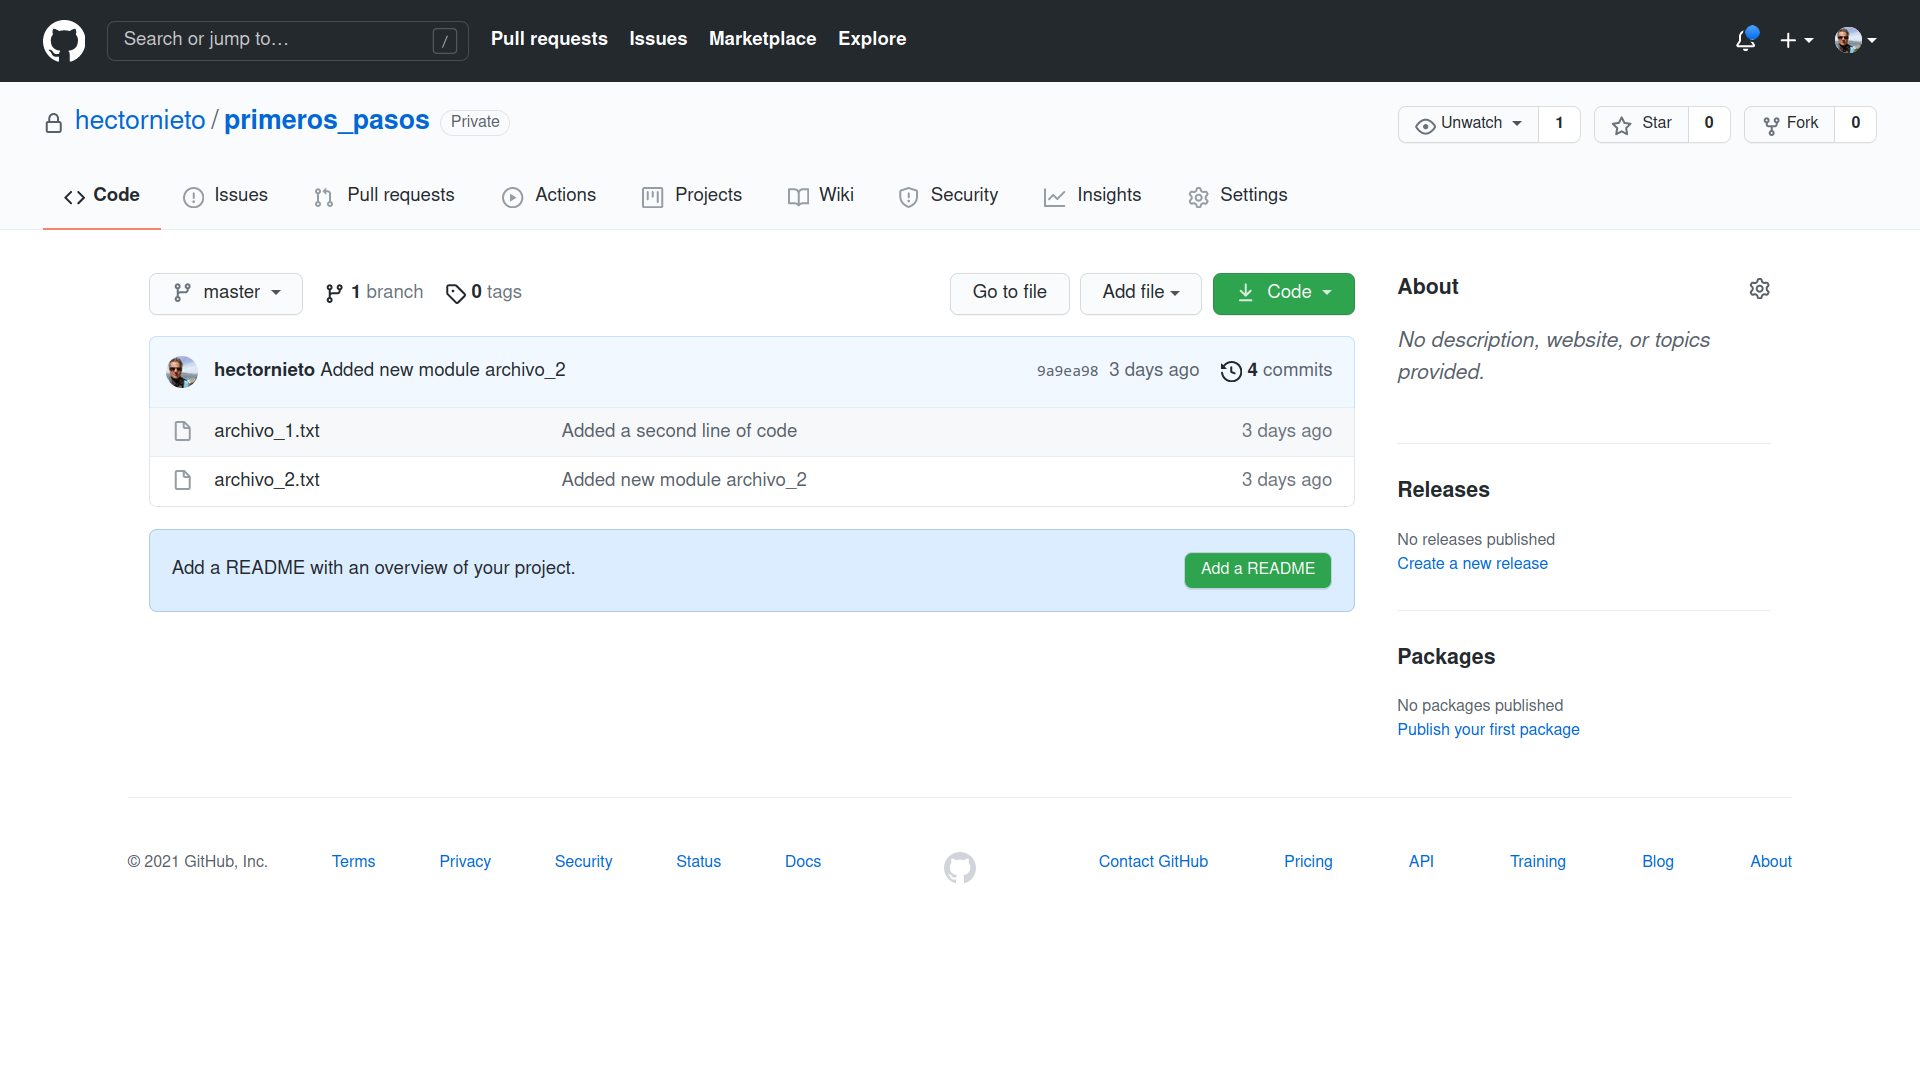
\includegraphics[width=\textwidth]{github_add_readme}
      \end{figure}´
      
      \item Verás que GitHub te está mandando un mensaje para añadir un README y documentar el repositorio, vamos a hacerle caso y pinchar en el botón verde \cverb+Add a README+. Aparecerá un editor de texto para escribir texto libre, en formato Markdown. Escribe una pequeña descripción, por ejemplo que tú eres el autor y que se trata de un curso. Puedes pinchar en \cverb+Preview+ para ver cómo se mostraría en la pantalla inicial de tu repositorio en GitHub. Cuando estés contento guarda el archivo pinchando abajo del todo en \cverb+Commit new file+ dejando el resto de las opciones por defecto. En seguida el navegador volverá a la pantalla de inicio y verás que el repositorio de GitHub contiene ya el nuevo archivo \verb+README.md+
      
      \item Ahora lo que ocurre es que en tu remoto tienes un commit (el nuevo archivo README.md) que no está en tu repositorio local. Por tanto acabamos con esta parte sincronizando ambos repositorios mediante el comando \verb+git pull+\footnote{git push sube los cambios realizados en local al remoto, mientras que git pull se podría decir que hace el camino inverso}. Para ello vuelve a tu terminal y teclea 
      
      \verb+git pull <alias_del_remoto> <branch>+. 
      
      Como es un repositorio privado siempre te va a pedir que te identifiques con tu usuario y contraseña. Si todo va bien tendrías que recibir un mensaje parecido a este:
      
      \begin{lstlisting}[style=custom]
Username for 'https://github.com': hectornieto
Password for 'https://hectornieto@github.com': 
remote: Enumerating objects: 4, done.
remote: Counting objects: 100% (4/4), done.
remote: Compressing objects: 100% (3/3), done.
remote: Total 3 (delta 0), reused 0 (delta 0), pack-reused 0
Unpacking objects: 100% (3/3), 752 bytes | 752.00 KiB/s, done.
From https://github.com/hectornieto/primeros_pasos
 * branch            master     -> FETCH_HEAD
   9a9ea98..bb74ee6  master     -> origin/master
Updating 9a9ea98..bb74ee6
Fast-forward
 README.md | 2 ++
 1 file changed, 2 insertions(+)
 create mode 100644 README.md
      \end{lstlisting}
      y verás que en tu carpeta local ya tienes el archivo README.md y verás que se ha incorporado el nuevo commit tecleando \cverb+git log+
      
      \item Prueba a subir y sincronizar otra de las ramas que has creado para familiarizarte con el trabajo sincronizado. Prueba también a añadir nuevos ediciones y commits en tus ramas locales y a subirlas con git push al remoto.
    \end{enumerate}
  
  \subsection{Control de cambios y versionado}
    Imagínate ahora que tu código tenía un error o bug, vamos a tener que editar de nuevo el archivo que creamos con una línea y corregir tu(s) línea(s) del código para que funcione correctamente. 
    
    \begin{enumerate}
    \item Para ello vuelve a editar el archivo y sobre-escribe el texto que habías escrito por este otro:
    \begin{cverbatim}
mi primera linea de codigo corregida
    \end{cverbatim}
      
    \item De nuevo para ver qué está pasando y cómo lo interpreta \verb+Git+ teclea \cverb+git status+
    
    \begin{lstlisting}[style=custom]
On branch master
Changes not staged for commit:
  (use "git add <file>..." to update what will be committed)
  (use "git restore <file>..." to discard changes in working directory)
	modified:   archivo_1.txt

no changes added to commit (use "git add" and/or "git commit -a")
    \end{lstlisting}
    
    Ahora te está diciendo que hay cambios en tu proyecto que aún no han sido añadidos para su posterior registro. Bien puedes ejecutar \cverb+git add <archivo>+ para añadir esos cambios al siguiente registro o descartar los mismos mediante \cverb+git restore <archivo>+. Nosotros, como estamos seguros y hemos visto que esta parte de código funciona queremos añadir y registrar el cambio. Pero antes vamos a asegurarnos qué es lo que ha cambiado entre la versión actual y la que fue registrada por el primer commit. 
    
    \item Teclea \cverb+git diff <archivo>+, un texto similar a este te aparecerá
    
    \begin{lstlisting}[style=custom, language=diff]
diff --git a/archivo_1.txt b/archivo_1.txt
index 7aa40b1..b3c9105 100644
--- a/archivo_1.txt
+++ b/archivo_1.txt
@@ -1 +1 @@
-mi primera linea de codigo
+mi primera linea de codigo corregida
    \end{lstlisting}
    donde las partes en rojo indican líneas que han sido eliminadas y las partes en verde muestran líneas que han sido añadidas.
    
    \item Repite los pasos 3 y 4 para añadir la nueva versión del archivo y registrarla bajo un nuevo commit. Recuerda modificar el comentario del commit para que refleje de forma clara el porqué de tal cambio, p.ej: 
    
    \cverb+git commit -m 'Fix initial bug'+
    
    \item Añade ahora una segunda línea de código (cualquier frase serviría) a nuestro archivo y guárdalo. Crea un nuevo archivo de texto (p.ej. \verb+archivo_2.txt+) con algún contenido (cualquier texto valdría). Si tecleas ahora \cverb+git status+ te aparecería un mensaje diciéndote por un lado que el archivo que ya habías registrado ha sido modificado y, por otro lado, que hay un nuevo archivo que aún no ha sido añadido para el seguimiento.
    
    \begin{lstlisting}[style=custom]
On branch master
Changes not staged for commit:
  (use "git add <file>..." to update what will be committed)
  (use "git restore <file>..." to discard changes in working directory)
	modified:   archivo_1.txt

Untracked files:
  (use "git add <file>..." to include in what will be committed)
	archivo_2.txt

no changes added to commit (use "git add" and/or "git commit -a")
    \end{lstlisting}
    
    \item Añade ambos archivos para registrar un nuevo commit.  \cverb+git add+ permite añadir varios archivos a la vez, e incluso también permite añadir un conjunto de archivos usando ``wildcards'', por ejemplo teclea \cverb+git add archivo_*+ para añadir todos los archvios existentes en tu carpeta que comiencen por \verb+archivo_+. Teclea de nuevo \cverb+git status+
    
    \begin{lstlisting}[style=custom]
On branch master
Changes to be committed:
  (use "git restore --staged <file>..." to unstage)
	modified:   archivo_1.txt
	new file:   archivo_2.txt
    \end{lstlisting}    
    verás que \verb+Git+ te está diciendo que hay cambios listos para ser registrados con un nuevo \verb+commit+. Estos cambios se resumen en que hay un archivo existente que ha sido modificado y un nuevo archivo añadido.
    
    \item Llegados a este punto, nos hemos dado cuenta que en realidad el segundo archivo que hemos creado no funciona correctamente, o simplemente no lo queremos incluir en esta nueva versión. Podemos descartar su inclusión antes de hacer el commit tecleando \cverb+git restore --staged archivo_2.txt+ o también tecleando \cverb+git reset archivo_2.txt+. Vuelve a teclear \cverb+git status+ para ver de nuevo el estado actual:
    
    \begin{lstlisting}[style=custom]
On branch master
Changes to be committed:
  (use "git restore --staged <file>..." to unstage)
	modified:   archivo_1.txt

Untracked files:
  (use "git add <file>..." to include in what will be committed)
	archivo_2.txt
    \end{lstlisting}
    
    \item Crea ahora un nuevo commit y ponle de nuevo un comentario útil y descriptivo para la nueva versión, p.ej. \cverb+git commit -m 'Added a second line of code'+
    
    \item Ahora sí, hemos visto que el segundo archivo o módulo funciona como queremos y queremos añadirlo al proyecto. Por lo tanto lo añadimos para el siguiente commit y lo registramos:
    \begin{cverbatim}
git add archivo_2.txt
git commit -m 'Added new module archivo_2'
    \end{cverbatim}
    
    \item Asegúrate que no tienes ningua tarea pendiente mediante \cverb+git status+. Si todo va sobre ruedas el entorno de trabajo debería estar limpio:
    
    \begin{lstlisting}[style=custom]
On branch master
nothing to commit, working tree clean
    \end{lstlisting}
    
    \item Vamos ahora a comprobar y revisar la historia de nuestro código mirando las distintas versiones que hemos realizado. Para ello en primer lugar teclea \cverb+git log+ para ver un registro detallado de todos los commits que has hecho, mostrando el identificador único de cada commit, el autor y la fecha del registro y el comentario/significado del mismo:

    \begin{lstlisting}[style=custom]

commit 9a9ea9821aed745099708b9f4e551b5516425c5a (HEAD -> master)
Author: hectornieto <hector.nieto.solana@gmail.com>
Date:   Sun May 9 11:53:12 2021 +0200

    Added new module archivo_2

commit f0cf4797ed331ee16d2ac5efe23a41f250436f0f
Author: hectornieto <hector.nieto.solana@gmail.com>
Date:   Sun May 9 11:50:28 2021 +0200

    Added a second line of code

commit 062ccfc2447929add19a36cf6b898b91bd005c90
Author: hectornieto <hector.nieto.solana@gmail.com>
Date:   Sun May 9 11:20:48 2021 +0200

    Fix inital bug

commit ba43a6b0218f5812cd6d4f445231c13819f4bb19
Author: hectornieto <hector.nieto.solana@gmail.com>
Date:   Sun May 9 10:39:02 2021 +0200

    My first commit
    \end{lstlisting}
    
    Por otro lado, con \cverb+git log --oneline+ obtenemos una salida resumida y más fácil de ver del mismo historial:
    \begin{lstlisting}[style=custom]
9a9ea98 (HEAD -> master) Added new module archivo_2
f0cf479 Added a second line of code
062ccfc Fix inital bug
ba43a6b My first commit
    \end{lstlisting}
    con el id del commit y su descripción.
    
    El verdadero potencial que tiene git es que guarda un registro del estado de cada uno de los archivos que hayamos añadido nuestro proyecto, por lo que podemos analizar y restaurar todas y cada una de las versiones que hayamos resgistrado con \verb+git commit+.
    
    \item Vamos entonces a comprobar las diferencias de contenido entre la versón actual y la de veriones anteriores. Para ello usaremos el comando \verb+git diff+, que admite distintas posibilidades. 
    \begin{itemize}
      \item Podemos ver diferencias entre la versión actual y las anteriores mediante \cverb+git diff HEAD~<número>+ donde el número nos indica el número de commits anteriores al actual. Por ejemplo teclea 
      \cverb+git diff HEAD~1+ 
      para ver los cambios entre la versión actual y la previa:
      \begin{lstlisting}[language=diff]
diff --git a/archivo_2.txt b/archivo_2.txt
new file mode 100644
index 0000000..01a59b0
--- /dev/null
+++ b/archivo_2.txt
@@ -0,0 +1 @@
+lorem ipsum
      \end{lstlisting}
      
      \item También podemos ver diferencias entre commits usando sus \verb+id+. Con \cverb+git log --oneline+ anota los id de dos de los commits e introdúcelos en el comando \cverb+git diff <commit_1> <commit_2>+. En mi caso si quisiera ver qué ha cambiado entre el primer commit (\verb+ba43a6b My first commit+) y mi último commit, tendría que teclear \cverb+git diff ba43a6b 9a9ea98+
      
      \begin{lstlisting}[language=diff]
diff --git a/archivo_1.txt b/archivo_1.txt
index 7aa40b1..ac6c5fc 100644
--- a/archivo_1.txt
+++ b/archivo_1.txt
@@ -1 +1,2 @@
-mi primera linea de codigo
+mi primera linea de codigo corregida
+segunda linea de codigo
diff --git a/archivo_2.txt b/archivo_2.txt
new file mode 100644
index 0000000..01a59b0
--- /dev/null
+++ b/archivo_2.txt
@@ -0,0 +1 @@
+lorem ipsum

      \end{lstlisting}
      
    \end{itemize}
    \end{enumerate}
  \subsection{Restaurar versiones previas}
    El gran interés que tiene \verb+Git+ es poder restaurar cualquier versión previa de los archivos/códigos que hayamos registrado. Hay varias formas pero la más recomendable como iniciación es con \verb+git checkout+.
    
    De igual modo que con \verb+diff+, \verb+checkout+ puede usarse mediante el id del commit o en relativo a partir del número de commits previos al estado actual (llamado \verb+HEAD+)\
    \begin{enumerate}
      \item Ejecuta \cverb+git checkout HEAD~2+ para restaurar la antepenúltima versión (también puedes usar \cverb+git checkout <commit>+, donde \verb+<commit>+ sería el id del antepenúltimo commit.
      
      \begin{lstlisting}[style=custom]
Note: switching to 'HEAD~2'.

You are in 'detached HEAD' state. You can look around, make experimental
changes and commit them, and you can discard any commits you make in this
state without impacting any branches by switching back to a branch.

If you want to create a new branch to retain commits you create, you may
do so (now or later) by using -c with the switch command. Example:

  git switch -c <new-branch-name>

Or undo this operation with:

  git switch -

Turn off this advice by setting config variable advice.detachedHead to false

HEAD is now at 062ccfc Fix inital bug
    \end{lstlisting}
      
    \item Teclea ahora \verb+git log --oneline+ para confirmar que estás en el commit que querías. Si todo va según lo planeado, mira ahora el contenido de la carpeta, verás que el segundo archivo que añadimos en el último commit ya no está. Además si abres el primer archivo éste no contendrá las modificaciones hechas en los dos últimos commits. En este punto podrías correr tu código con esa versión e incluso hacer nuevas modificaciones al mismo a partir de ese estado. Sin embargo, no te preocupes y no entres en pánico, siempre puedes volver a la última versión tecleando \cverb+git checkout -+ o \cverb+git checkout <branch>+, donde \verb+branch+ es la rama (por defecto \verb+master+) en la que estabas trabajando. Verás que los archivos vuelven a estar según estaban en el último commit que hicimos\footnote{Git almacena todo el historial desde la creación del proyecto (con git init) por lo que puedes revisar y restaurar todos y cada uno de las versiones que hayas registrado con git commit}.

    \item Hay otros dos comandos que hacen tareas similares:     
    
    \cverb+git reset <commit>+ es mucho más agresivo al eliminar directamente los registro posteriores a \verb+<commit>+. Es una herramienta que a veces se usa para ``reescribir'' la historia\footnote{Lo de reescribir la historia mejor lo dejamos para los políticos nacionalistas, vengan de donde vengan} del repositorio borrando permanentemente los cambios realizados posteriores, y por tanto no se recomienda utilizar cuando el repositorio está ligado a un repositorio remoto, por ejemplo en GitHub. El otro comando, que es más recomendable es \cverb+git revert <commit>+, que restaurará todo el código una versión anterior y ese cambió quedará registrado como un nuevo commit, por lo tanto una manera mucho más transparente y recomendable para restaurar versiones en códigos compartidos.
    
   \end{enumerate}
   
  \subsection{Ramificaciones del código}
    En esta sesión trabajaremos con conceptos algo más avanzados que es posible que no necesites a estas alturas, pero extremadamente útiles cuando tienes ya desarrollado un código estable o quieras/necesites trabajar con un código de terceros, y deseas hacer alguna modificación siginicativa sin correr el riesgos de liarla parda. Para ello nos familiarizarmos con el uso de ramificaciones de código y fusionados de ramas. Esto sería la antesala del trabajo de git colaborativo, donde varios desarrolladores trabajan bajo un mismo repositorios a la vez y sugieren cambios al dueño/gestor del repositorio, también comúnmente llamado el ``Benevolente dictador del código''.
    
    \begin{enumerate}
     \item Continuamos desde donde lo dejamos en la sección anterior, es decir debemos tener dos archivos de texto, uno con las siguientes dos líneas:
     \begin{lstlisting}[style=custom]
mi primera linea de codigo corregida
segunda linea de codigo
     \end{lstlisting}
     
     y otro con la siguente línea
     
    \begin{lstlisting}[style=custom]
lorem ipsum
    \end{lstlisting}
    
    \item Asumamos que este es un código ya maduro y puesto en producción, es decir operativo. Pero hay algunas modificaciones o ideas que pueden que sean necesarias pero puede que no estés seguro de que funcionen, o a lo mejor tu supervisor se ha obsesionado que cambies o añadas un análisis y para mantenerlo contento lo intentarás implementar aun sabiendo que prácticamente es una pérdida de tiempo. Es por ello que no quieres manosear inútilmente tu rama principal del código. Para eso creamos una nueva ramificación del mismo desde la base de la última versión registrada. En la carpeta de tu repositorio teclea
    
    \cverb+git branch dev+
    
    donde \verb+dev+ es el nombre de la rama que le hemos dado, aunque puedes darle cualquier otro nombre que se te ocurra y que sea más auto-explicativa (p.ej. \verb+capricho_del_jefe+)
    
    \item puedes ver ahora las ramas de tu código tecleando \cverb+git branch+, apareciendo resaltado con un asterisco (y distinto color) el nombre de la rama en la que te encuentras actualmente
    
    \begin{lstlisting}[style=custom]
  dev
* master
    \end{lstlisting}

    \item cambia de rama tecleando \cverb+git checkout dev+ o con \cverb+git switch dev+.
    
    \begin{lstlisting}[style=custom]
Switched to branch 'dev'
    \end{lstlisting}
    
    si tecleas \cverb+git log+ o \cverb+git log --oneline+ verás que tenemos los mismos commits que con tu rama maestra, y si echas un ojo al contenido de tus archivos aparecen exactamente como estaban en master. Es decir ambas ramas en este momento son exactamente idénticas.
    
    \item Asegúrate que estas en la rama dev (con \cverb+git branch+) y edita el segundo archivo, añadiendo una segunda línea \cverb+nueva linea experimental+. Guarda el archivo, y registra el cambio\footnote{Recuerda que los cambios se registran primero añadiendo archivos al futuro commit con git add para despues confirmar y documentar el cambio con git commit}.
    
    \item mira ahora la lista de commits con \cverb+git log --oneline+. Algo similar a esto debería aparecerte:
    
    \begin{lstlisting}[style=custom]
deb0b98 (HEAD -> dev) Include more effiicent computation
9a9ea98 (master) Added new module archivo_2
f0cf479 Added a second line of code
062ccfc Fix inital bug
ba43a6b My first commit
    \end{lstlisting}

    \verb+Git+ te está indicando que hasta el penúltimo commit todos provienen de la rama master, a partir de la cual esta rama (\verb+dev+) tiene un nuevo commit \verb+deb0b98 (HEAD -> dev) Include more effiicent computation+ que ya no forma parte de \verb+master+.
    
    \item Regresa de nuevo a tu rama \verb+master+ tecleando \cverb+git checkout master+, y vuelve a teclear \cverb+git log --oneline+, ¿ves la diferencia? Echa un ojo también al contenido del \verb+archivo_2+, que acababas de editar, y verás que ha retornado a ser idéntico a como estaba antes de la rama \verb+dev+. Puedes ir cambiando entre todas las ramas que tengas y \verb+Git+ restaurará el contenido de los archivos y el historial de versiones tal y como estaba registrada por última vez.
    
    \item Trabajar con ramificaciones puede ser un poco locura en proyectos grandes o con varios colaboradores. Es por ello que hay herramientas para visualizar el historial del proyecto \verb+Git+ con todas sus ramificaciones. En este tutorial miraremos dos maneras, aunque hay infinidad de interfaces gráficas de \verb+Git+ que permiten de una manera u otra realizar visualizaciones similares
    \begin{itemize}
     \item teclea: 
     
     \hspace{-2cm}\cverb+git log --oneline --graph --all --simplify-by decoration+
     
     para ver en la terminal una visualización simplificada de todas las ramificaciones de tu código. Ya conocemos qué hace \verb+git log --oneline+, en este caso le añadimos la opción \verb+graph+ para que muestre en la terminal en forma de gráfico, \verb+all+ para que muestre todas las ramas a la vez, y  \verb+simplify-by decoration+ para que sólo muestre los registros relevantes, es decir, aquéllos cuando ocurrieron las ramificaciones.
     
     \item Otra forma más amigable de ver la evolución de las ramificaciones es en GitHub, claro está siempre que esté en esta plataforma. Vamos a echar un ojo al estado de uno de mis repositorios (\verb+pyTSEB+) en GitHub. 
     En tu explorador navega a \url{https://github.com/hectornieto/pyTSEB}, pincha en \verb+Insights+ y luego \verb+Network+ para ver un gráfico similar a este
     \begin{figure}[H]¯
      \hspace{-1cm}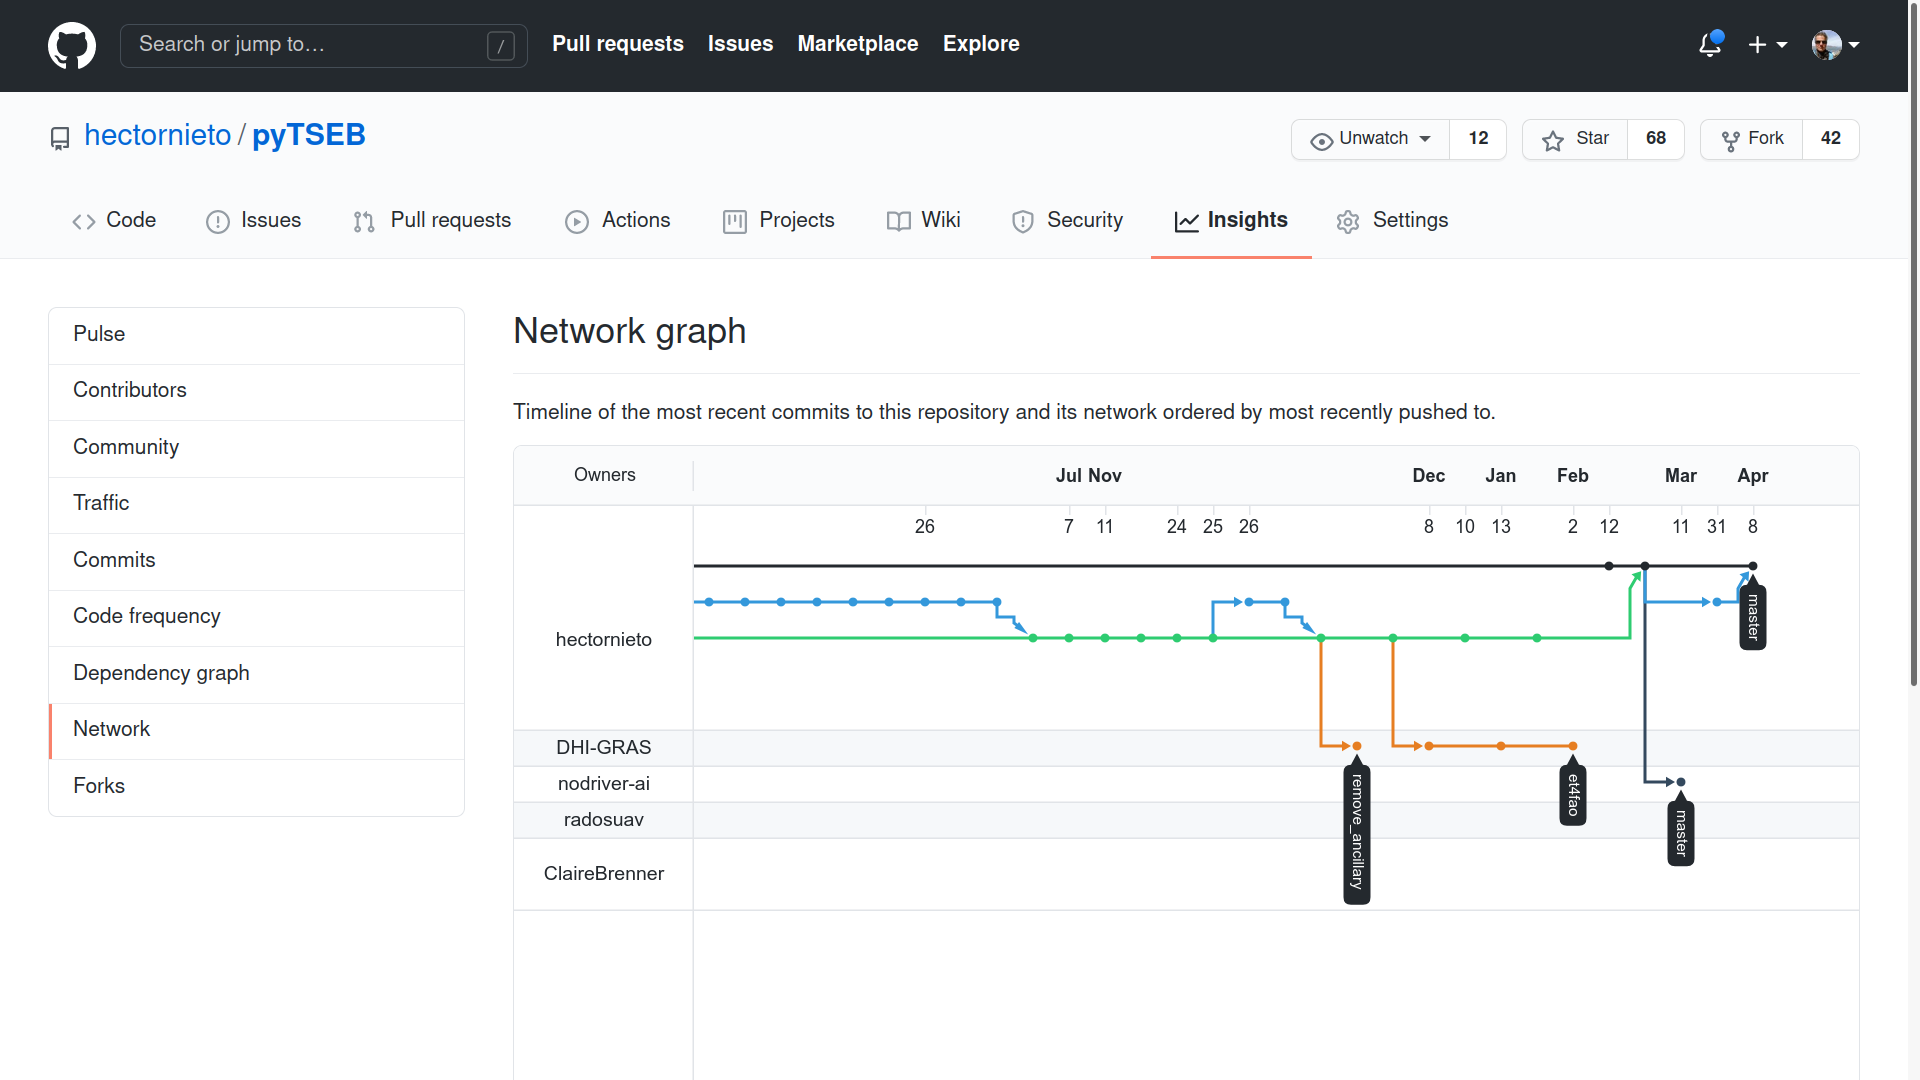
\includegraphics[width=1.2\columnwidth]{pyTSEB_branches}
     \end{figure}
    \end{itemize}

    \item Haz nuevas ramas y nuevos commits a lo loco y expermienta con todas las herramientas hechas hasta ahora. Por ejemplo prueba a ver los efectos de \verb+git reset+, \verb+git revert+ y \verb+git checkout+ para entender mejor las diferentes formas de restaurar vesiones previas del código. Lo bueno que tienen las ramas es que puedes experientar con cambios en tu código sin afectar la rama principal donde tienes la versión estable del mismo así que haz cosas, en libertad, sin miedo\footnote{En una sola frase he conseguido plagiar a M. Rajoy, Ayuso y Pablo Iglesias}.
    \end{enumerate}
 
   \subsection{Actualizar el repositorio  local y remoto}
    Antes de irnos a la cama, y tras una jornada dura de picar código ha llegado el momento de guardar nuestro código en la nube para tenerlo seguro, y así también poder acceder al mismo desde cualquier lado sin tener que llevarlo en un pendrive. Es aquí donde los repositorios remotos, es decir plataformas tipo GitHub, juegan su rol principal, aparte de ser, en un futuro próximo, el escaparate donde colguéis vuestros códigos y software para la comunidad científica y/o el público en general.
    
    Vamos a actualizar las dos ramas con la que hemos estado trabajando. 
    \begin{enumerate}
    
     \item Empecemos con la rama \verb+dev+. Asegúrate que en el terminal que la rama dev es la rama activa\footnote{Recordatorio: git branch te dice qué ramas hay y cuál es la rama activa, y git switch <branch>  cambia entre ramas}. \verb+dev+ aún no tiene una rama hermana en el remoto por lo que tenemos que crearla y subir los contenidos mediante
     
     \cverb+git push -u origin dev+
     
     Es decir crea una rama llamada \verb+dev+en el repositorio remoto con alias \verb+origin+ y sube los contenidos de mi rama actual\footnote{Es recomendable, por simplicidad usar el mismo nombre para las ramas locales y remotas}. Debería aparecer un mensaje similar a este:
     \begin{lstlisting}[style=custom]
Username for 'https://github.com': hectornieto
Password for 'https://hectornieto@github.com': 
Enumerating objects: 5, done.
Counting objects: 100% (5/5), done.
Delta compression using up to 4 threads
Compressing objects: 100% (2/2), done.
Writing objects: 100% (3/3), 332 bytes | 332.00 KiB/s, done.
Total 3 (delta 0), reused 0 (delta 0)
remote: 
remote: Create a pull request for 'dev' on GitHub by visiting:
remote:      https://github.com/hectornieto/primeros_pasos/pull/new/dev
remote: 
To https://github.com/hectornieto/primeros_pasos
 * [new branch]      dev -> dev
Branch 'dev' set up to track remote branch 'dev' from 'origin'.
     \end{lstlisting}

     
     \item \verb+Master+ ya tiene su rama remota en creada, que hicimos en la sección \ref{sec:sincronizar}, por lo que para subir el contenido de tu repositorio local al GitHub no hace falta incluir las opciones \verb+-u <alias_del_remoto> <rama_del_remoto>+, y como ya por defecto +Master+ tiene un rama asignada en el remoto para su seguimiento. ´
     
     Cambia de rama con \cverb+git switch master+ o \cverb+git checkout master+, y teclea \cverb+git push+ para actualizar los contenidos de \verb+Master+.
     
    \end{enumerate}
      
    Ya sabes el manejo básico de Git y GitHub. El resto del tutorial lo dedicaremos a tareas más específicas dentro del trabajo colaborativo, pero ya estás preparado/a para realizar el 99\% de las tareas con Git que necesitarás, por lo que ya puedes subir versionar tus propios códigos  y subirlos a GitHub, bien para compartirlos en público o mantenerlos en privado para tener siempre una copia en la nube.

  \section{Fusión y resolución de conflictos}
  \subsection{Fusionados de ramificaciones}
    El fin último de trabar con ramas es incorporar en tu rama principal el código que hayas desarrollado, una vez hayas visto que funciona y que es estable. Para eso hay dos nuevos comandos que vamos a aprender \cverb+git rebase+ y \cverb+git merge+.
    
    \begin{enumerate}
     \item Empecemos por ver de nuevo el estado de nuestras ramas, teclea
     
     \cverb+git log --oneline --all --graph+
     
     para ver la evolución de las mismas. Algo similar a esto debería aparecer:
     
     \begin{lstlisting}[style=custom]
* bb74ee6 (origin/master, master) Create README.md
| * deb0b98 (HEAD -> dev, origin/dev) Include more effiicent computation
|/  
* 9a9ea98 Added new module archivo_2
* f0cf479 Added a second line of code
* 062ccfc Fix inital bug
* ba43a6b My first commit
     \end{lstlisting}
    
    Al principio cuesta visualizarlo pero muestra que tenemos dos ramas que se bifurcan: \verb+origin/master+ y \verb+master+ son las ramas principales (la remota y la local) en la que contiene el archivo \verb+REAMDE.md+ que creamos desde \verb+GitHub+. Por otro lado temeos la rama \verb+dev+, tanto en local como en remoto(\verb+origin/dev+), que se bifurcó de \verb+master+ tras añadir \verb+archivo_2.txt+ (en este ejemplo es el commit \verb+9a9ea98+) y que incluye un registro que no está en \verb+master+ (\verb+deb0b98+ en este ejemplo). 
    
    Cuando estamos trabajando con ramas, y sobre todo cuando queremos incorporar los cambios realizados en una rama en la rama principal, es conveniente tener actualizada la rama que estamos desarrollando con las últimas actualizaciones de la rama principial\footnote{Imagínate que tienes tu software ya en producción (rama principal, llamémosle version 1.0) pero ya estás trabajando con la versión 2.0 en otra rama. Mientras trabajas en la nueva versión es posible que otros usuarios o tú mismo te des cuenta de la existencia de algunos bugs y/o pequeñas mejoras que hacer en la versión 1.0, por lo que añades nuevos commits a la rama principal, teniendo así la version 1.1. Llegados a este punto te interesa que la rama sobre la que estás desarrollando la versión 2.0 incorpore también esos cambios}. Esto se hace con el comando \cverb+git rebase master+.
    
    \item Activa la rama \verb+dev+ mediante \cverb+git switch dev+ o \cverb+git checkout dev+
    
    \item Antes de hacer la actualización, y para que veas mejor lo que va a pasar haz una nueva rama a partir de \verb+dev+ con:
    \cverb+git branch dev_old+
    
    \item teclea de nuevo 
    \cverb+git log --oneline --all --graph+
    para ver que la nueva rama que has creado se encuentra en el mismo estado que \verb+dev+
    
    \begin{lstlisting}[style=custom]
* bb74ee6 (origin/master, master) Create README.md
| * deb0b98 (HEAD -> dev, origin/dev, dev_old) Include more effiicent computation
|/  
* 9a9ea98 Added new module archivo_2
* f0cf479 Added a second line of code
* 062ccfc Fix inital bug
* ba43a6b My first commit
    \end{lstlisting}
    
    \item Ahora actualiza \verb+dev+ al último registro de la rama \verb+master+ mediante
    
    \cverb+git rebase master+
    
    Que viene a indicar resitúa mi rama actual al último commit de la rama master. Vuelve a ejecutar 
    
    \cverb+git log --oneline --all --graph+ 
    
    para ver la situación de cada una de las ramas tras el rebase. También mira el contenido de tu repositorio para cada una de las ramas y las diferencias entre ellas.
   
    \end{enumerate}
    
    Ahora que ya tenemos re-actualizada nuestra rama en desarrollo con la última versión de la rama principal, podemos seguir trabajando mejorando nuestro código o incorporar definitivamente los cambios a la rama \verb+master+. Para esto último se utiliza el comando \verb+git merge+. \cverb+git merge <branch>+  indica al sistema que coja la rama \cverb+<branch>+ y la fusione en la rama actual
    
    \begin{enumerate}
     \item Queremos fusionar la rama \verb+dev+ en la rama \verb+master+, por lo que primero de todo tenemos que activar la rama \verb+master+
     \cverb+git switch master+
     \item Ya estando en la rama que queremos actualizar mediante el fusionado, teclea
     \cverb+git merge dev+
     
     Como anteriormente habíamos hecho un rebase de dev a master, el fusionado se tendría que hacer sin problemes y un mensaje similar a este debería aparecer
     \begin{lstlisting}[style=custom]
Updating bb74ee6..cdd9770
Fast-forward
 archivo_2.txt | 2 ++
 1 file changed, 2 insertions(+)
     \end{lstlisting}
     
     \item Ahora \verb+master+ tiene todos los cambios y actualizaciones hechas en \verb+dev+, por lo que ambas ramas son idénticas y, de hecho podríamos eliminar \verb+dev+. Teclea 
     \cverb+git branch -D dev+ para borrar definitivamente \verb+dev+ de tu repositorio local, aunque seguirá existiendo en tu repositorio remoto. Para eliminar ramas del remoto, por ejemplo de GitHub, puedes hacerlo directamente desde la web de GitHub o mediante el comando \cverb+git push <alias_del_remoto>  --delete <rama_del_remoto>+.

    \end{enumerate}
    
    Si te fijas de nuevo en el mensaje que recibiste al ejecutuar \verb+git merge dev+, La actualización/fusionado se ha realizado mediante la estrategia \verb+Fast Forward+, que significa que simplemente git puede añadir todos los registros nuevos al final del último registro. Esto es debido a que previamente al fusionado hicimos una actualización de la rama \verb+dev+ para que incluyese todos los commits de \verb+master+ posteriores al momento en que ambas ramas se separaron. Esto a veces no siempre es posible y, sobre todo al actualizar/sincronizar los repositorios remotos, que han podido sufrir cambios desde otro ordenador o por otro usuarios. 
    
    Afortunadamente \verb+Git+ es suficientemente inteligente para decidir qué estrategia de fusionado es la mejor para cada caso (según los registros en común y las divergencias entre ramas), por lo que no te tienes que preocupar mucho de esto\footnote{Sobre todo para el nivel de programación al que aspiramos}. Sin embargo, puede darse el caso, y más frecuente de lo que te imaginas sobre todo en las fases de iniciación de \verb+Git+, que haya casos en los que el sistema no pueda hacer la fusión de forma automática, y entonces es cuando tenemos nosotros que resolver el conflicto.
  
  \subsection{Resolución de conflictos}
    Un conflicto es debido a que al hacer ejecutar ua actualización de ramas, bien sea por \verb+merge+, \verb+rebase+ o \verb+pull+ hay líneas del código que han sido modificadas en las dos ramas y discrepan en su contenido. En estos casos, que pueden ser bastante probables si no hacemos fusionados y actualizacoines con el remoto frecuentes. Cuando esto ocurre \verb+Git+ avisa que no ha podido completar el fusionado por la existencia de conflictos y nos pide que manualmente los solucionemos.
    
    Vamos a generar voluntariamente un conflicto y ver lo que pasa y los pasos a seguir para resolverlo:
    \begin{enumerate}
     \item Partimos de la situación anterior, en la que tenemos una rama \verb+master+ con los cambios de \verb+dev+ ya incorporados.
     
     \item Crea una nueva rama y llámala por ejemplo \verb+futuro_conflicto+:
     \cverb+branch futuro_conflicto+
     
     \item con la rama \verb+master+ activada edita uno de los arhivos de texto (por ejemplo \verb+archivo_1.txt+) y añade una línea con este texto
     \cverb+nueva linea de codigo de la rama master+
     
     \item Registra el cambio en un nuevo commit, p.ej.
     \begin{cverbatim}
git add archivo_1.txt
git commit -m 'master conflicting commit'
     \end{cverbatim}

     \item cambia ahora a la rama \verb+futuro_conflicto+ y edita el mismo archivo\footnote{verás que al estar un commit por detrás de master la linea que recientemente editaste no aparece} con esta linea
     
     \cverb+nueva linea de codigo en futuro_conflicto+
     
     \item registra el cambio en un nuevo commit, p.ej.
     \begin{cverbatim}
git add archivo_1.txt
git commit -m 'futuro_conflicto conflicting commit'
     \end{cverbatim}
     
     \item Echa un ojo ahora a las diferencias entre las dos ramas
     
     \cverb+git diff futuro_conflicto master+

    \begin{lstlisting}[language=diff]
diff --git a/archivo_1.txt b/archivo_1.txt
index 7230ec3..16094fb 100644
--- a/archivo_1.txt
+++ b/archivo_1.txt
@@ -1,3 +1,3 @@
 mi primera linea de codigo corregida
 segunda linea de codigo
-nueva linea de codigo en futuro_conflicto
+nueva linea de codigo de la rama master
    \end{lstlisting}
    Verás que sólo difieren en una línea.
    
    \item Ahora vamos a intentar fusionar la rama \verb+futuro_conflicto+ en \verb+master+. Activa la rama \verb+master+ y teclea
    
    \cverb+git merge futuro_conflcto+
    
    Recibirás un mensaje parecido a este:
    \begin{lstlisting}[style=custom]
Auto-merging archivo_1.txt
CONFLICT (content): Merge conflict in archivo_1.txt
Automatic merge failed; fix conflicts and then commit the result.
    \end{lstlisting}
    Que viene a decir que \verb+Git+ no puede por sí solo fusionar las ramas por la existencia de conflictos en el \verb+archivo_1.txt+. Nos pide que arreglemos el conflicto y que registremos el cambio.
    
    \item Edita de nuevo el archivo en conflicto, verás que presenta un texto similar a este:
    
    \begin{lstlisting}[style=custom]
mi primera linea de codigo corregida
segunda linea de codigo
<<<<<<< HEAD
nueva linea de codigo de la rama master
=======
nueva linea de codigo en futuro_conflicto
>>>>>>> futuro_conflicto
    \end{lstlisting}
    
    \verb+Git+ te está indicando dónde y en qué modo está el conflcto. Tenemos que resolvor todo el texto que está entre \verb+<<<<<<<+ y \verb+>>>>>>>+, de modo que lo que hay entre \verb+<<<<<<< HEAD+ y \verb+=======+ es la parte conflictiva que pertenece al último commit (\verb+HEAD+) de la rama actual (\verb+master+), y lo que está entre \verb+=======+ y es la parte conflictiva que hay en la rama \verb+futuro_conflicto+.
    
    \item Edita manualmente el texto de modo que tu código final se ajuste a lo que realmente querías, por ejemplo podemos pensar que la parte de \verb+master+ es la buena, o viceversa, o incluso que ninguna de las dos líneas es la correcta y reescribir esa línea.
    
    \item Una vez termines y estés satisfecho con la resolución del conflicto tu texto no debería contener ningún caracter del tipo \verb+<<<<<<<+, \verb+>>>>>>>+ o \verb+=======+. Por ejemplo:
  
    \begin{lstlisting}[style=custom]
mi primera linea de codigo corregida
segunda linea de codigo
nueva linea de codigo con conflicto resuelto
    \end{lstlisting}
    
    Podemos guardar el archivo y cerrarlo.
    
    \item Ya tenemos el archivo como nos gustaría que quedase tras la fusión, para continuar con la misma tendemos que volver a añadirlo al espacio de trabajo:
    \cverb+git add archivo_1.txt+
    
    \item Opcionalmente podemos registrar el conflicto con un nuevo commit
    
    \item Esto lo repetiríamos para cualquier otro conflicto que tengamos, una vez todos estén resueltos y añadios al espacio de trabajo podemos continuar con la fusión mediante
    
    \cverb+git merge --continue+
    Si no has registrado commits durante esta fase, al ejecutar este último comando \verb+Git+ te daraá la opción de editar el texto del commit, puedes dejar ese texto por defecto o modificarlo.
    
    ¡Enhorabuena! ya ha solucionado tu primer conflicto durante una fusión. Si bien los pasos a realizar durante un conflicto siempre son los mismos: editar los archivos conflictivos, añadirlos al espacio de trabajo y continuar el fusionado mediante el keyword (\verb+--continue+), no hay ninguna regla sobre cómo resolver los mismos\footnote{si la hubiera Git ya habría hecho el fusionado automáticamente}, y cada caso que se te presente será distintos y tendrás que apelar al sentido común y al objetivo que tenga la(s) linea(s) de código conflictivas.
     
    \end{enumerate}

  \section{Código colaborativo en GitHub}
   En esta última tarea vais a subir vuestros progresos a mi repositorio del curso (\url{https://github.com/hectornieto/cursoGit}), con el fin de poder certificar a la UAH vuestro aprovechamiento del curso.
   
   A la hora de trabajar en un equipo o incluso sugerir cambios en el repositorio de un tercero no es recomendable hacerlo directamente en el repositorio original. El proceso típico es hacer una copia (\verb+Fork+) en tu cuenta GitHub, hacer los cambios necesarios y hacer un \verb+Pull Request+ desde tu repositorio GitHub hacia el repositorio original.
   
   \subsection{Creación de copias (``Forks'')}
  \begin{enumerate}
   \item Primero vamos a descargar y sincronizar el repositorio del curso a una carpeta de tu PC. Teclea
   
   \cverb+git clone https://github.com/hectornieto/cursoGit+
   Un mensaje parecido a éste aparecerá 
   
   \begin{lstlisting}[style=custom]
Cloning into 'cursoGit'...
remote: Enumerating objects: 72, done.
remote: Counting objects: 100% (72/72), done.
remote: Compressing objects: 100% (49/49), done.
remote: Total 72 (delta 29), reused 60 (delta 20), pack-reused 0
Unpacking objects: 100% (72/72), 13.05 MiB | 9.12 MiB/s, done.
   \end{lstlisting}
   y tendrás un repositorio local del curso en la carpeta \cverb+cursoGit+. Si tienes tiempo y ganas, puedes ver todos los commits que se han hecho para preparar el curso, desde que se inició el repositorio.
   
   \item Teclea \cverb+git remote -v+ para confirmar que el repositorio ya está ligado al repositorio remoto con alias \verb+origin+.
   
   \begin{lstlisting}[style=custom]
origin	https://github.com/hectornieto/cursoGit (fetch)
origin	https://github.com/hectornieto/cursoGit (push)
   \end{lstlisting}
   
   \item Abre tu navegador y ve al repositorio cursoGit de GitHub: \url{https://github.com/hectornieto/cursoGit}. Asegúrate de ingresar en GitHub con tu usuario y contraseña, y pincha en el botón \cverb+Fork+ de la parte superior derecha.
   
   \item Ahora ve a tu cuenta GitHub y verás que tienes en tu GitHub una copia del repositorio del curso. Si miras a través de las distintas ramas del repositorio verás en primer lugar que he creado una rama por cada uno de vosotros, y al pinchar en cada una de ellas aparecerá un mensajito que dice \verb+This branch is even with hectornieto:<branch>+. Normal, porque de momento acabamos de hacer la copia.
   
   \item Vuelve al terminal de tu PC y añade también la copia remota de tu GitHub a tu repositorio local con:
   
   \hspace{-3cm}\cverb+git remote add <alias_del_remoto> https://github.com/<usuario>/cursoGit+
   
   Donde \cverb+<alias_del_remoto>+ podría ser cualquier nombre excepto \verb+origin+ ya que este alias ya está asignado al repositorio de mi cuenta. Un nombre común en estos casos suele ser \cverb+upstream+.
   
   \item Confirma que tu repositorio local está ahora conectado a los dos repositorios remotos, el original al que más adelante haremos el \verb+Pull Request+ y su copia en tu propio espacio \verb+GitHub+, mediante el comando \cverb+git remote -v+
  
    \begin{lstlisting}[style=custom]   
origin	https://github.com/hectornieto/cursoGit (fetch)
origin	https://github.com/hectornieto/cursoGit (push)
upstream	https://github.com/complutig/cursoGit (fetch)
upstream	https://github.com/complutig/cursoGit (push)
    \end{lstlisting}
    \end{enumerate}
    
    La idea de tener dos remotos es usar el remoto original para tener siempre actualizado tus repositorios, tanto el  local como tu copia remota. Para ello se recomienda confirmar el estado de sincronización con \cverb+git status+ y en caso de que haya nuevos commits en el repositorio original traerlos a tus copias con \cverb+git pull origin <branch>+. Luego subir los cambios que hagas desde tu repositorio local a tu repositorio remoto, con el fin último de hacer el \verb+Pull Request+ desde tu remoto al remoto original.

    \subsection{Sugerencias de cambios (``Pull Request'')}
    Ya tenemos nuestra copia local y remoto. Ahora lo que vamos a hacer para terminar el curso es añadir todos los archivos que has creado en la práctica anterior al repositorio del curso. Para ello vas a trabajar con la rama asociada a tu nombre de usuario \verb+GitHub+.
    
    \begin{enumerate}
     \item Para asegurarnos que tenemos los últimos registros del repositorio original teclea \cverb+git fetch --all+
     
     \item Como hay una rama remota con tu nombre de usuario \verb+GitHub+ teclea \cverb+git checkout <usuario>+ para que el sistema construya esa rama en tu repositorio local.
     
     \item Crea una carpeta vacía llamada \cverb+ejercicio_<usuario>+ donde sustituye \cverb+<usuario>+ por tu nombre de usuario GitHub.
     
     \item Copia todo el repositorio de \verb+primeros_pasos+ a esta carpeta
     
     \item Añade esa carpeta y todo su contenido al sistema \verb+Git+ y registra el cambio con un commit
     
     \begin{cverbatim}
git add ejercicio_<usuario>
git commit -m <mensaje>
     \end{cverbatim}
     
     \item Sube los cambios a tu repositorio remoto con:
     
     \cverb+git push <alias_del_remoto> <branch>+
     
     donde \cverb+<alias_del_remoto>+ es el alias de tu remoto (p.ej. \cverb+upstream+) y \cverb+<branch>+ es el nombre de la rama que estás subiendo (que en este caso es el nombre de tu usuario \verb+GitHub+). SI todo va bien un mensaje similar a este debería aparecer
     
     \begin{lstlisting}[style=custom]
Username for 'https://github.com': hectornieto
Password for 'https://hectornieto@github.com': 
Enumerating objects: 3, done.
Counting objects: 100% (3/3), done.
Delta compression using up to 4 threads
Compressing objects: 100% (2/2), done.
Writing objects: 100% (2/2), 237 bytes | 237.00 KiB/s, done.
Total 2 (delta 1), reused 0 (delta 0)
remote: Resolving deltas: 100% (1/1), completed with 1 local object.
To https://github.com/complutig/cursoGit
5b0e2c6..f98d500  test -> test
     \end{lstlisting}
     
     \item Ahora que has subido los cambios a tu repositorio remoto puedes ir a tu cuenta \verb+GitHub+, navegar al repositorio \verb+cursoGit+ y activar la rama con tu nombre. Debería aparecer una pantalla con un mensaje similar a este:
     
     \begin{figure}[H]
      \hspace{-2cm}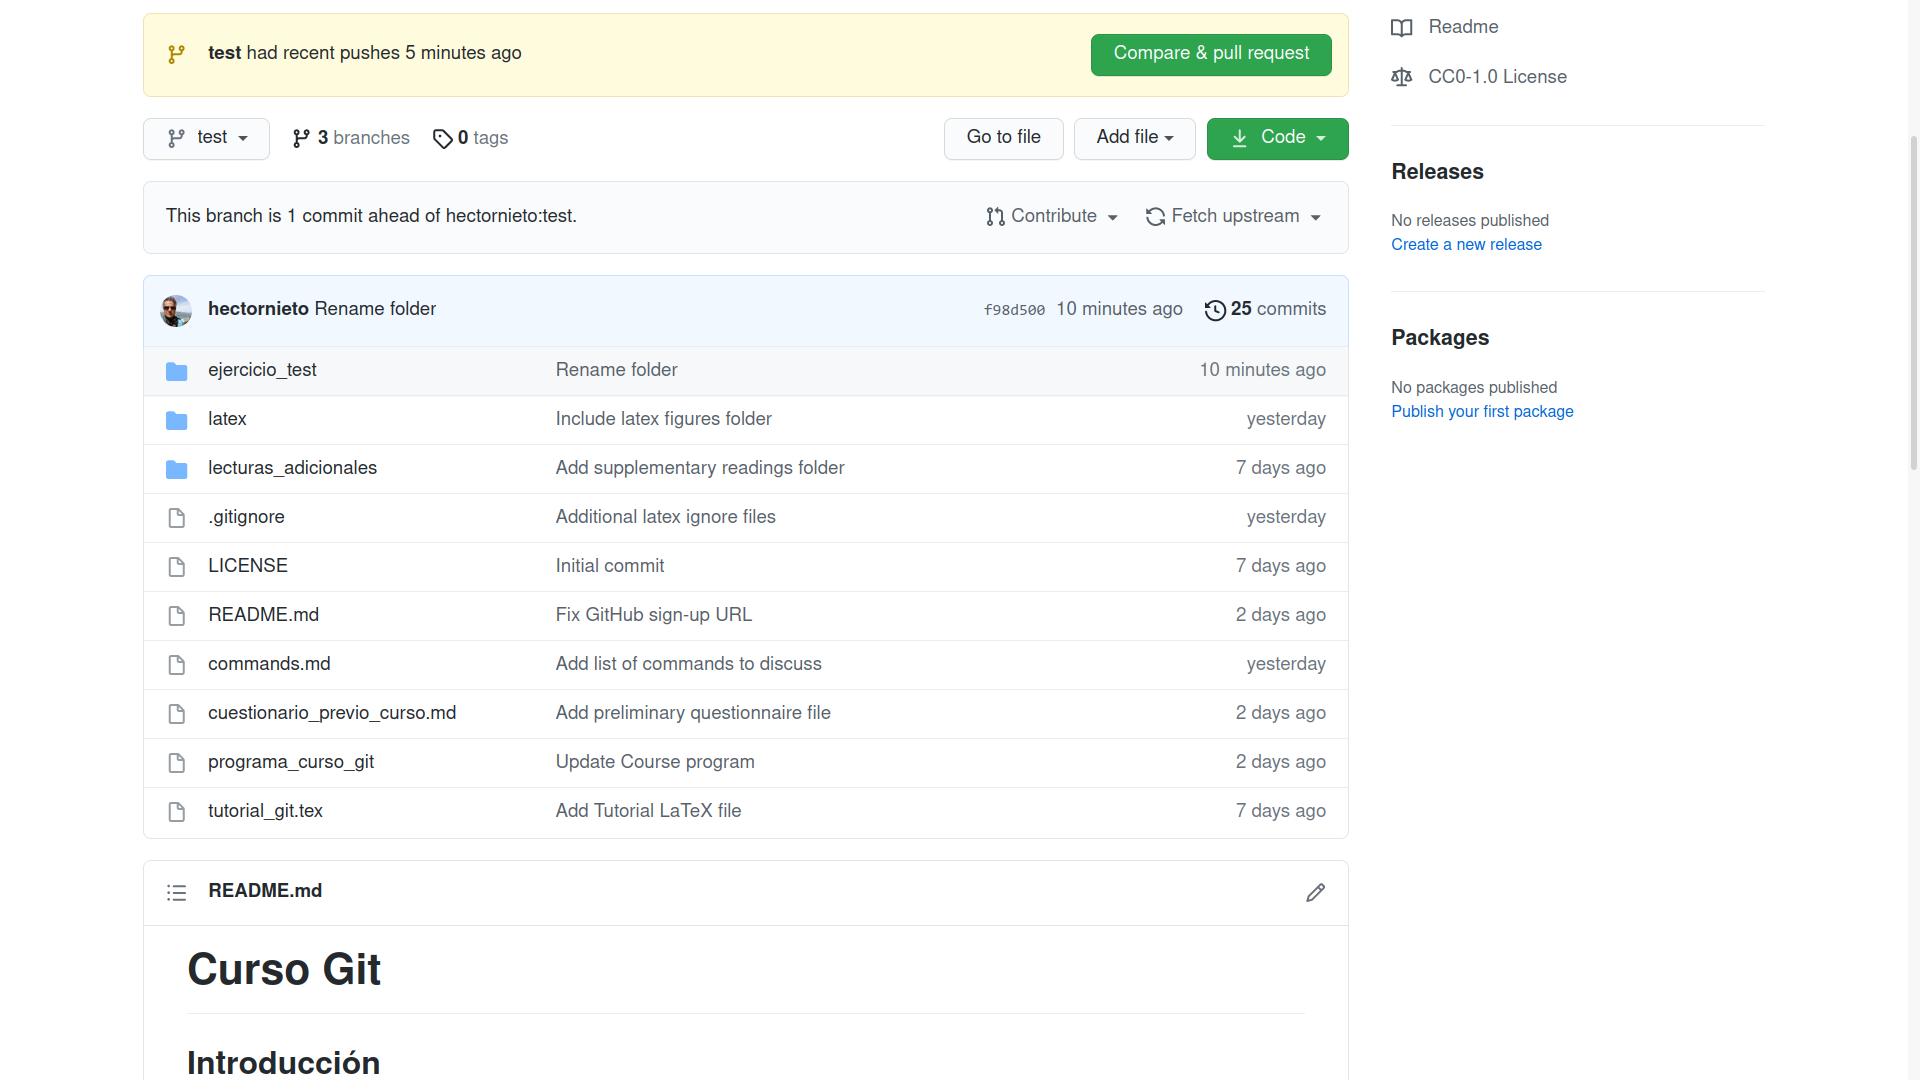
\includegraphics[width=1.6\columnwidth]{github_ready_for_pull_request}
     \end{figure}

    Como ves ya \verb+GitHub+ detecta que ha habido cambios entre la rama que tienes en tu repositorio remoto y la misma rama del repositorio original y te ofrece la posibilidad de comparar ambas ramas y hacer un pull request
    
    \item Pincha en el icono verde de \cverb+Compare & Pull Request+. Aparecerá una pantalla como esta
     \begin{figure}[H]
      \hspace{-2cm}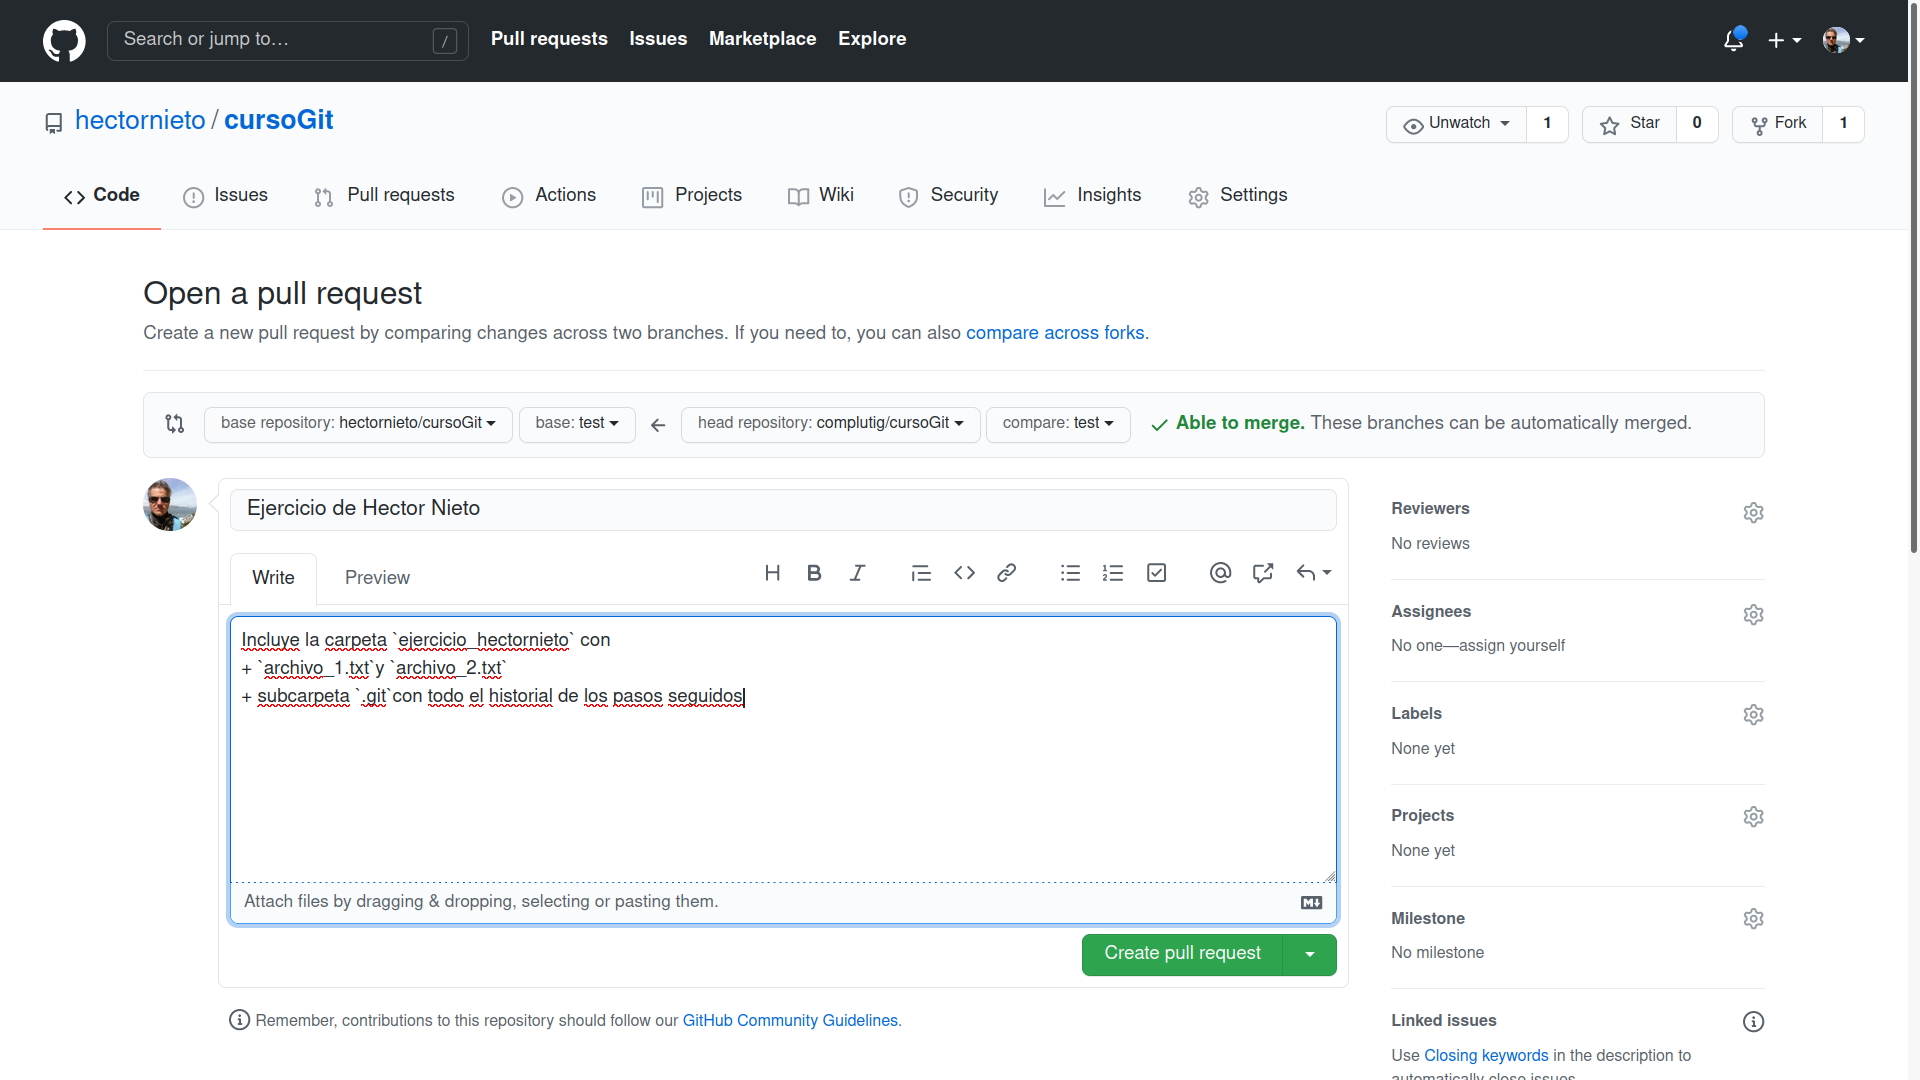
\includegraphics[width=1.4\columnwidth]{github_pull_request}
     \end{figure}
     
     En la que podrías modificar el repositorio base al que iría destinado el \verb+Pull Request+ y las ramas de origen y destino del mismo. En principio conviene revisar esto y en su caso modificar de acuerdo a lo que uno realmente quiera hacer. En el caso que nos atañe simplemente añade el nombre del \verb+Pull Request+, que generalemnte tiene que resumir en un a linea el por qué de la sugerencia del cambio (p.ej. \cverb+Ejercicio de <tu_nombre>+) y luego se suele añadir más detalles de los cambios en el cuadro de texto libre.
     
     \item Una vez completes el nombre y la descripción pincha en \cverb+Create pull request+ para finalizar con el proceso.

    \end{enumerate}
    
    ¡Enhorabuena! Has terminado con éxito este tutorial. Ahora te recomiendo que continúes practicando y empieces a crear repositorios con tu código, como ves \verb+Git+ es muy seguro y no deberías temer equivocarte porque siempre puedes volver a un estado previo.
    
    Una vez que haces un \verb+Pull Request+ a un repositorio de \verb+GitHub+, su dueño recibirá un e-mail con la notificación que tiene pendiente aprobar, comentar o rechazar la sugerencia. Si lo aprueba, el repositorio original se actualiza automáticamente con los cambios que sugeriste.
    
     \begin{figure}[H]
      \hspace{-1cm}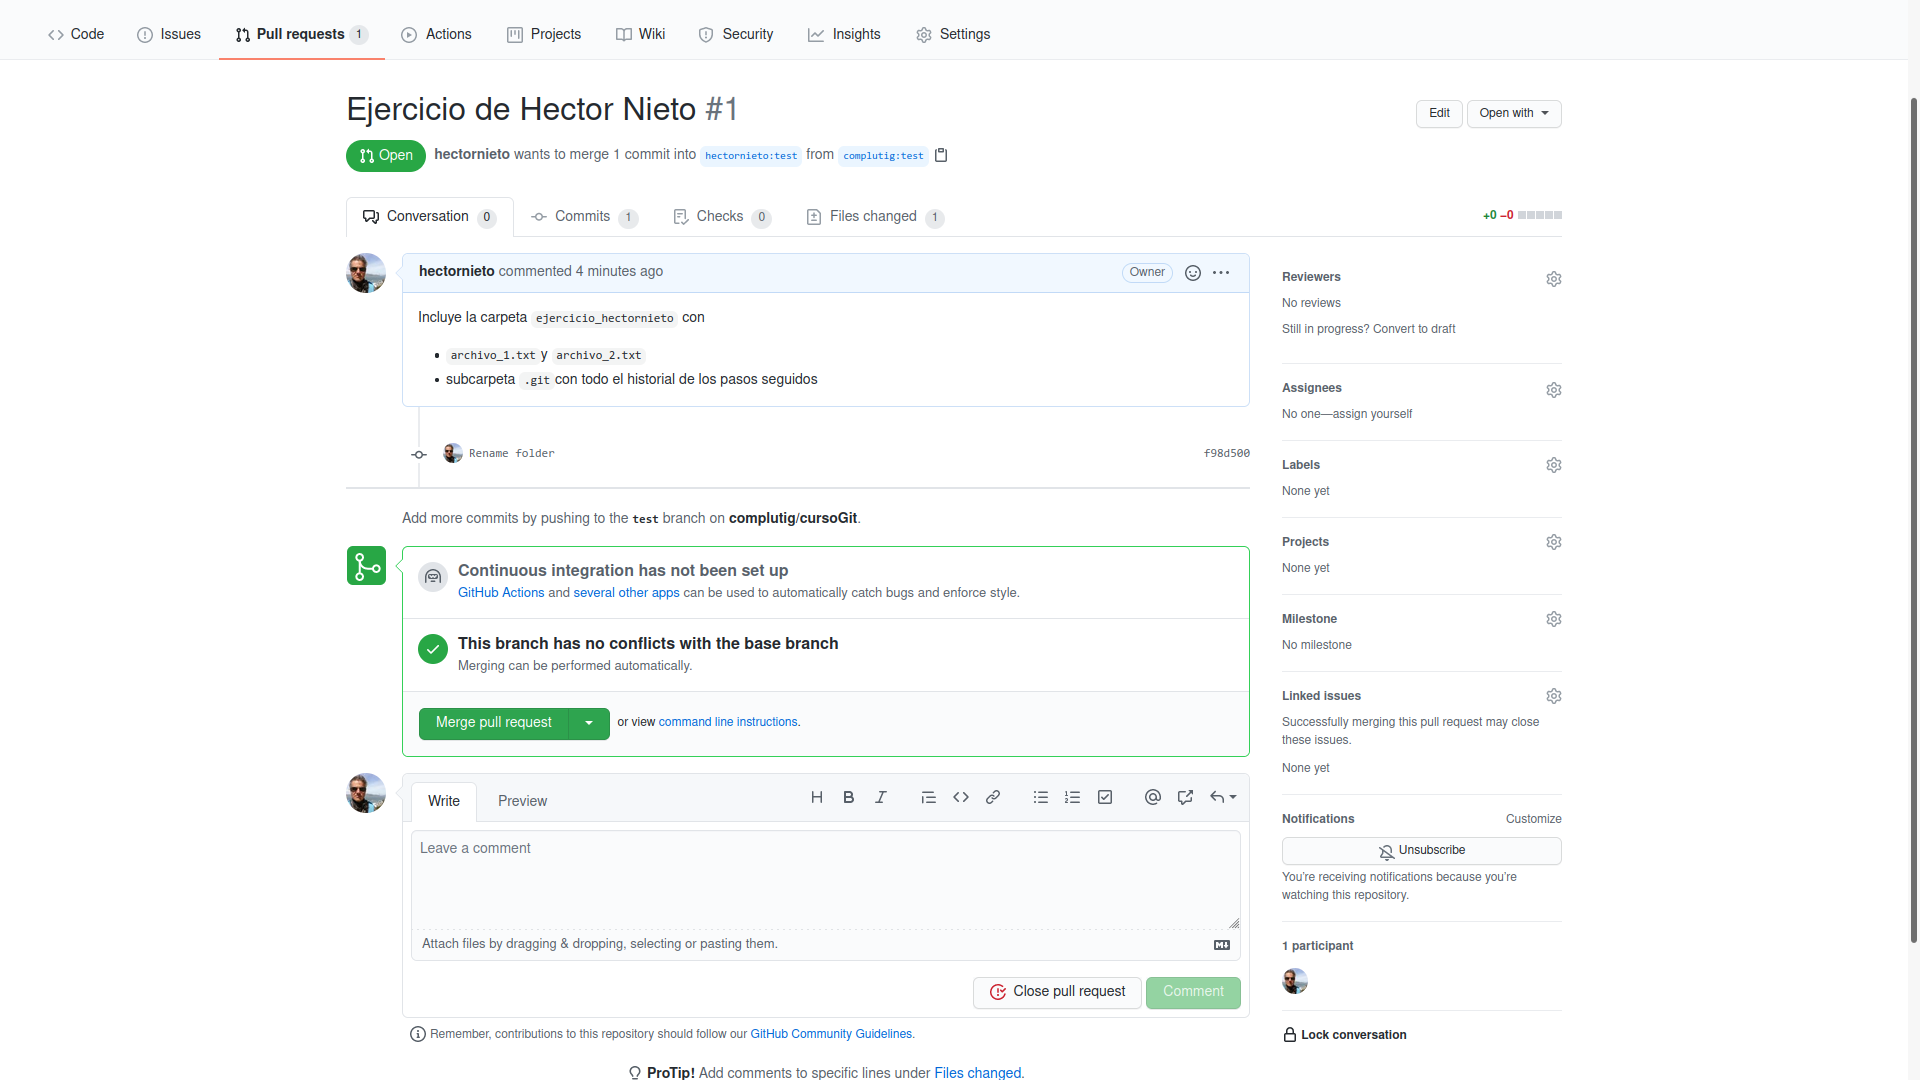
\includegraphics[width=1.6\columnwidth]{github_pending_pull_request}
      \caption{Ejemplo de Pull Request pendiente por aprobar por el dueño del repositorio}
     \end{figure}   
   

  \section{Descripción de los comandos de Git}
    \subsection{git init}
      Inicializa un repositorio git dentro de la carpeta actual. Al ejecutar \cverb+git init+ \verb+Git+ genera automáticamente una subcarpeta \verb+.git+ con todos los archivos del sistema de git. Puedes borrar un repositorio git simplemente borrando esta carpeta.
      
    \subsection{git add}
      Añade archivos o carpetas para ser registrados con \cverb+git comit+. \cverb+git add+ admite añadir de una sólo vez una serie de arhivos mediante su inclusión separados por espacios \cverb+git add <archivo_1> <archivo_2> <...>+. \cverb+git add+ también admite wildcards para añadir todos los archvos presentes en una carpeta que cumplan con un patrón en su nombre. Por ejemplo \cverb+git add *.py+ añadiría todos los arhivos dentro de la carpeta con la extensión \verb+.py+.
    
    \subsection{git commit}
      Confirma los cambios realizados tras \cverb+git add+ en una nueva versión (o commit). La forma más frecuente de utilizar este comando es con
      
      \cverb+git commit -m '<descripción_del_commit>'+
      
      donde es recomendable que \verb+<descripción_del_commit>+ sea un mensaje que identifique de manera concisa y clara los cambios realizados tras el último commit\footnote{Una buena práctica en programación y en Git es realizar commits lo más específicos posible, mejor muchos y cortos que un gran commit con muchos cambios dentro de los arhivos}. 
      
      El otro modo típico de utilizar este comando es con \cverb+git commit --amend+, que permite re-editar o actualizar el último commit realizado.
      
    \subsection{git diff}
    \cverb+git diff+ es el comando utilizado para visualizar diferencias entre versiones y archivos\footnote{Algo similar a la herramienta de control de cambios de Word}. Si tecleas \cverb+git diff+ a secas en el terminal el sistema de devuelve todas las modificaciones y diferencias que haya entre los archivos en su estado actual y la última versión registrada con \verb+commit+.
    
    Por otro lado, tecleando \cverb+git diff <archivo>+ \verb+Git+ permite visualizar las diferencias para un archivo en cuestión entre su versión actual y la última versión registrada con \verb+commit+.
    
    \cverb+git diff <commit_1> <commit_2>+ por otro lado te permite ver las diferencias entre dos versiones registradas
    
    También puedes usar 
    
    \cverb+git diff <commit_1> <commit_2> -- <archivo>+ 
    
    para ver las diferencias de un archivo entre dos versiones, o incluso 
    
    \cverb+git diff <branch_1> <branch_2> -- <archivo>+.
    
    para ver las diferencias de ese archivo entre dos ramas distintas.
    
    Finalmente también puedes comparar el estado de tus archivos entre tu repositorio local y remoto:
    
    \cverb+git diff <alias_del_remoto>/<branch_1> <branch_2> -- <archivo>+.
    
    Como ves las posibilidades y combinaciones para evaluar distintas versiones del código a lo largo del tiempo y en distintas ramas es infinita.
    
    \subsection{git checkout}
      Este comando es muy versátil y permite realizar distintos tipos de operaciones según el contexto en el que se aplique
      \begin{itemize}
       \item \cverb+git checkout <commit>+ o \cverb+git checkout HEAD~<número>+ permite restaurar una versión previa del repositorio
       \item \cverb+git checkout <branch>+ permite ir de una rama a otra.
       \item \cverb+git checkout <archivo>+ permite restaurar un archivo a su estado original, definido por el último commit.
      \end{itemize}
      
    \subsection{git branch}
      Se trata de operaciones para trabajar con ramificaciones. Estos son las operaciones y variantes del comando más típicas:
      
      \begin{itemize}
       \item \cverb+git branch+ proporciona un listado de ramificaciones existentes y señala la ramificación actual.
       \item \cverb+git branch <branch>+ crea una nueva rama con nombre \verb+<branch>+ como réplica de la ramificación en la que actualmente te encuentres.
       \item \cverb+git branch -D <branch>+ borra la rama de nombre \verb+<branch>+. Para poder borrar una ramificación tienes que hacerlo desde otra rama distinta.
      \end{itemize}
    
    \subsection{git merge}
    
    \subsection{git rebase}


 
\end{document}
